%!TEX root = ../main.tex

\newpage
\section*{Tables and Figures}

% Tables

  \begin{table}[H]
    \centering
    \caption{
      \textbf{Tools used in the \ac{micone} pipeline}.
      The tools highlighted in gray are the defaults for the pipeline that are recommended based on the benchmarks with the mock and synthetic datasets.
      The consensus algorithm in the Network Inference (\ac{ni}) step incorporates all the modules (bootstrapping, direct association, and correlation-based) to generate the consensus network.
    }
    \label{tab:micone_tools}
  \end{table}

% Figures

  % \FloatBarrier
  % \newpage
  % \begin{figure}[H]
  %   \centering
  %   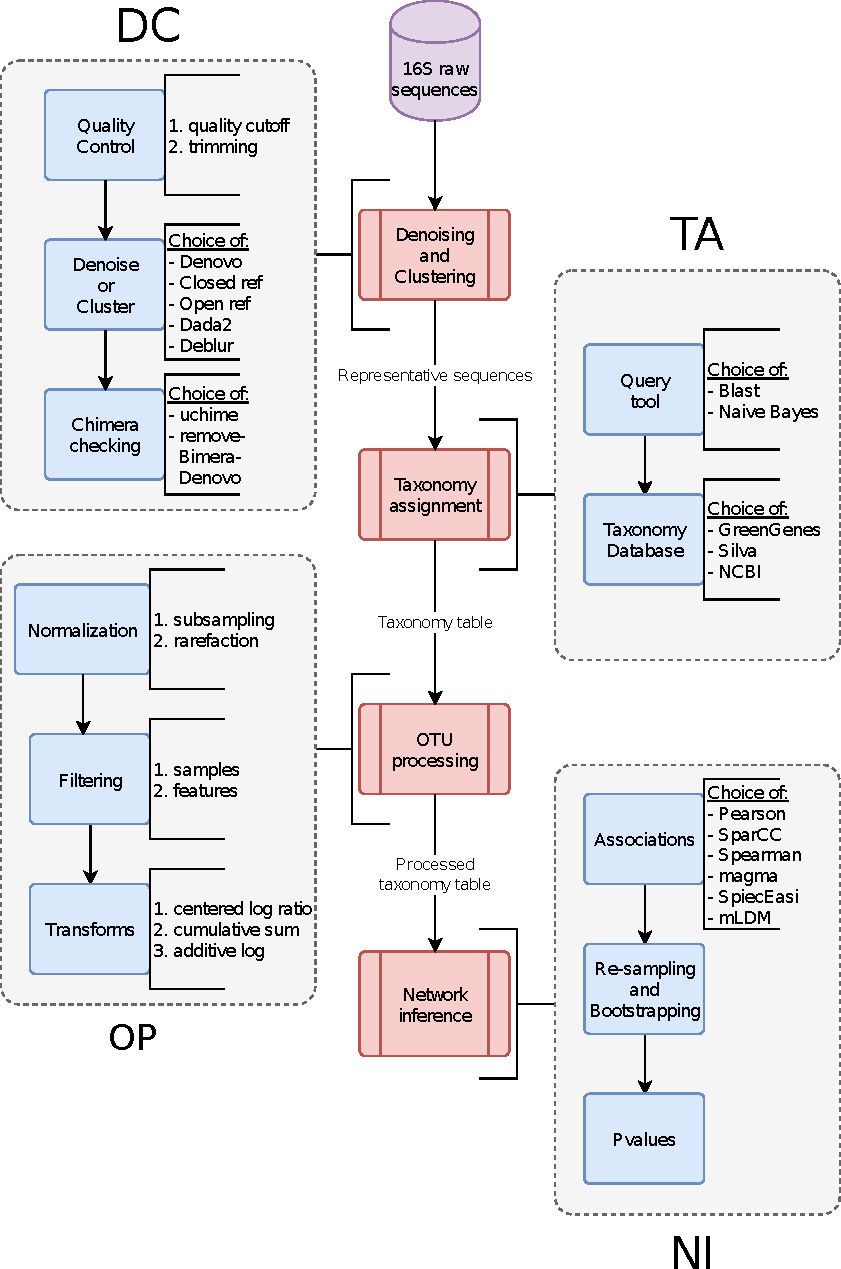
\includegraphics[width=0.74\linewidth]{figure1.pdf}
  % \end{figure}
  \begin{figure}[H]
    \centering
    \caption{
      \textbf{The workflow of the \ac{micone} pipeline}.
      The steps of the workflow can be broken down into five major groups: \textbf{(SP)} \textbf{S}equence \textbf{P}rocessing, \textbf{(DC)} \textbf{D}enoising and \textbf{C}lustering, \textbf{(TA)} \textbf{T}axonomy \textbf{A}ssignment, \textbf{(OP)} \textbf{O}TU and ESV \textbf{P}rocessing, and \textbf{(NI)} \textbf{N}etwork \textbf{I}nference.
      Each step incorporates several processes (blue boxes), each of which in turn has several alternative algorithms for the same task (indicated by the text to the right of the blue boxes).
      Each arrow describes the data that is being passed from one step to another.
      The inputs to the pipeline are 16S rRNA sequencing reads, and the final output is the consensus network generated from the inferred co-occurrence networks.
      For details on each process and the different outputs, see Methods.
    }
    \label{fig:figure1}
  \end{figure}



  % \FloatBarrier
  % \newpage
  % \begin{figure}[H]
  %   \centering
  %   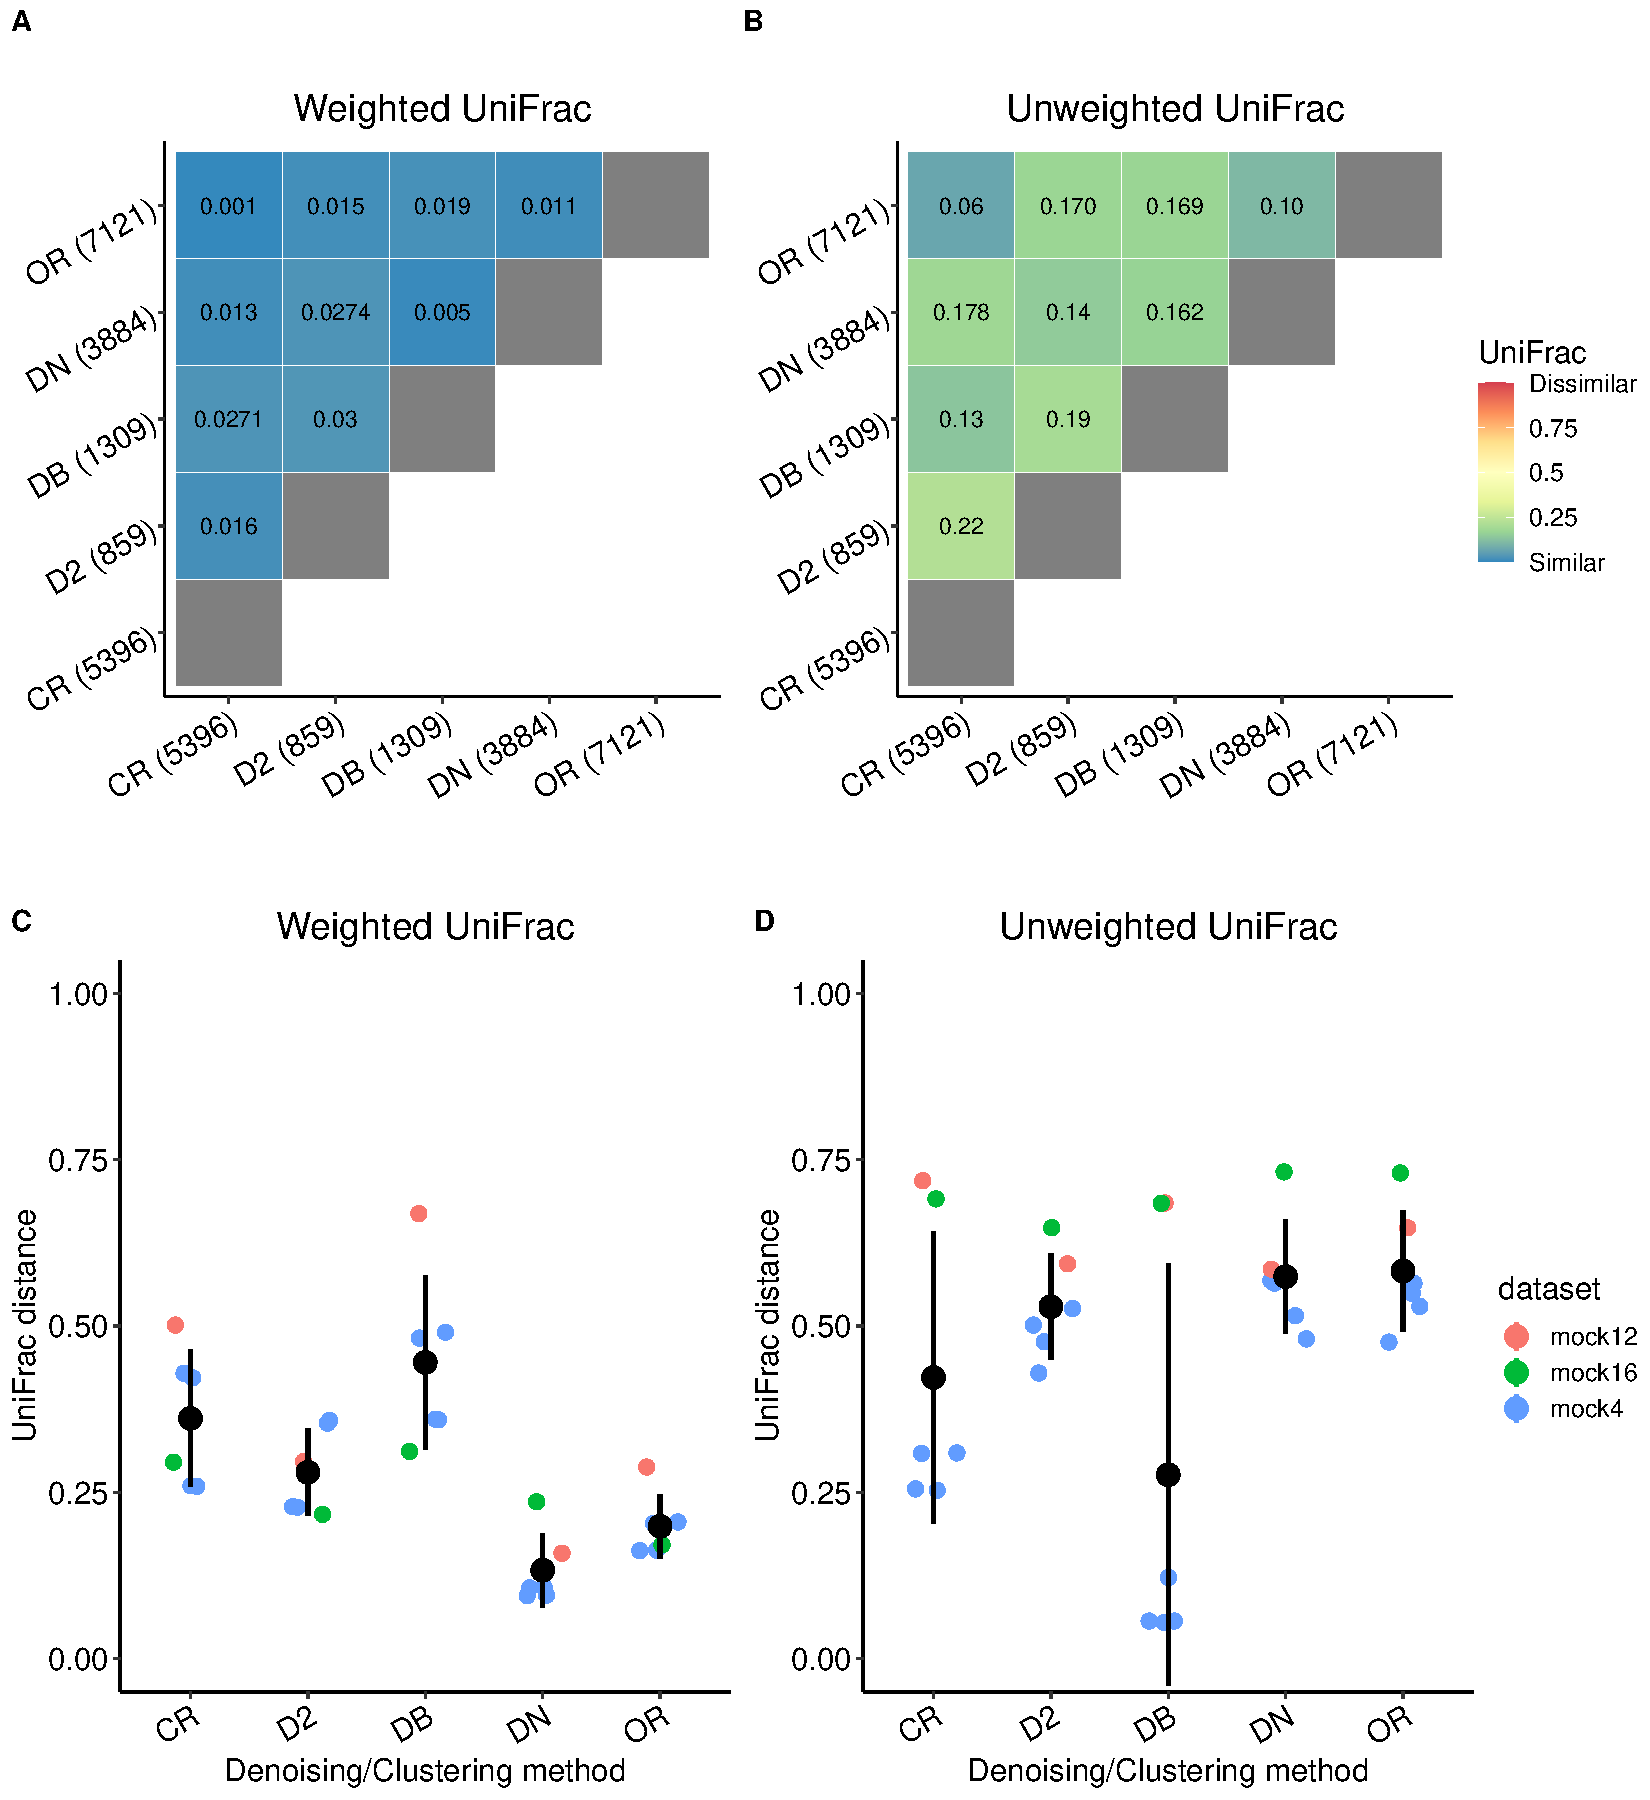
\includegraphics[width=\textwidth]{figure2.pdf}
  % \end{figure}
  \begin{figure}[H]
    \centering
    \caption{
      \textbf{The representative sequences generated by the different denoising and clustering methods differ in their identification of sequences that are low in abundance}.
      \textbf{(A)} The average weighted UniFrac distance between the representative sequences shows that the representative sequences and their compositions are fairly identical between the methods (with the exception of Deblur (DB) due to the low ESV count).
      \textbf{(B)} The relatively larger average unweighted UniFrac distance indicates that methods differ in their identification of sequences that are lower in abundance.
      The number of \ac{otu}s or \ac{esv}s generated by the respective methods are provided in the parenthesis next to their names.
      The data used for the analysis in (A, B) were the samples from the fecal microbiome transplant (FMT) dataset~\cite{Kang2017}, containing both healthy subjects and subjects with autism spectrum disorder (ASD).
      \textbf{(C, D)} The distributions of the average weighted and unweighted UniFrac distance between the predicted sequence profile and the expected sequence profile in the mock datasets.
      The average weighted UniFrac distances show that de novo (DN) and open reference (OR) were the best-performing methods in most of the datasets, while they are the worst-performing methods under the unweighted UniFrac metric.
      The good performance of dada2 (D2) under both distance metrics combined with its approach of identifying \ac{esv}s using de novo methods, prompts us to use it as the default method for the DC step.
      The data used for the analysis in (C, D) were the mock4, mock12, and mock16 datasets from mockrobiota~\cite{Bokulich2016}.
    }
    \label{fig:figure2}
  \end{figure}


  % \FloatBarrier
  % \newpage
  % \begin{figure}[H]
  %   \centering
  %   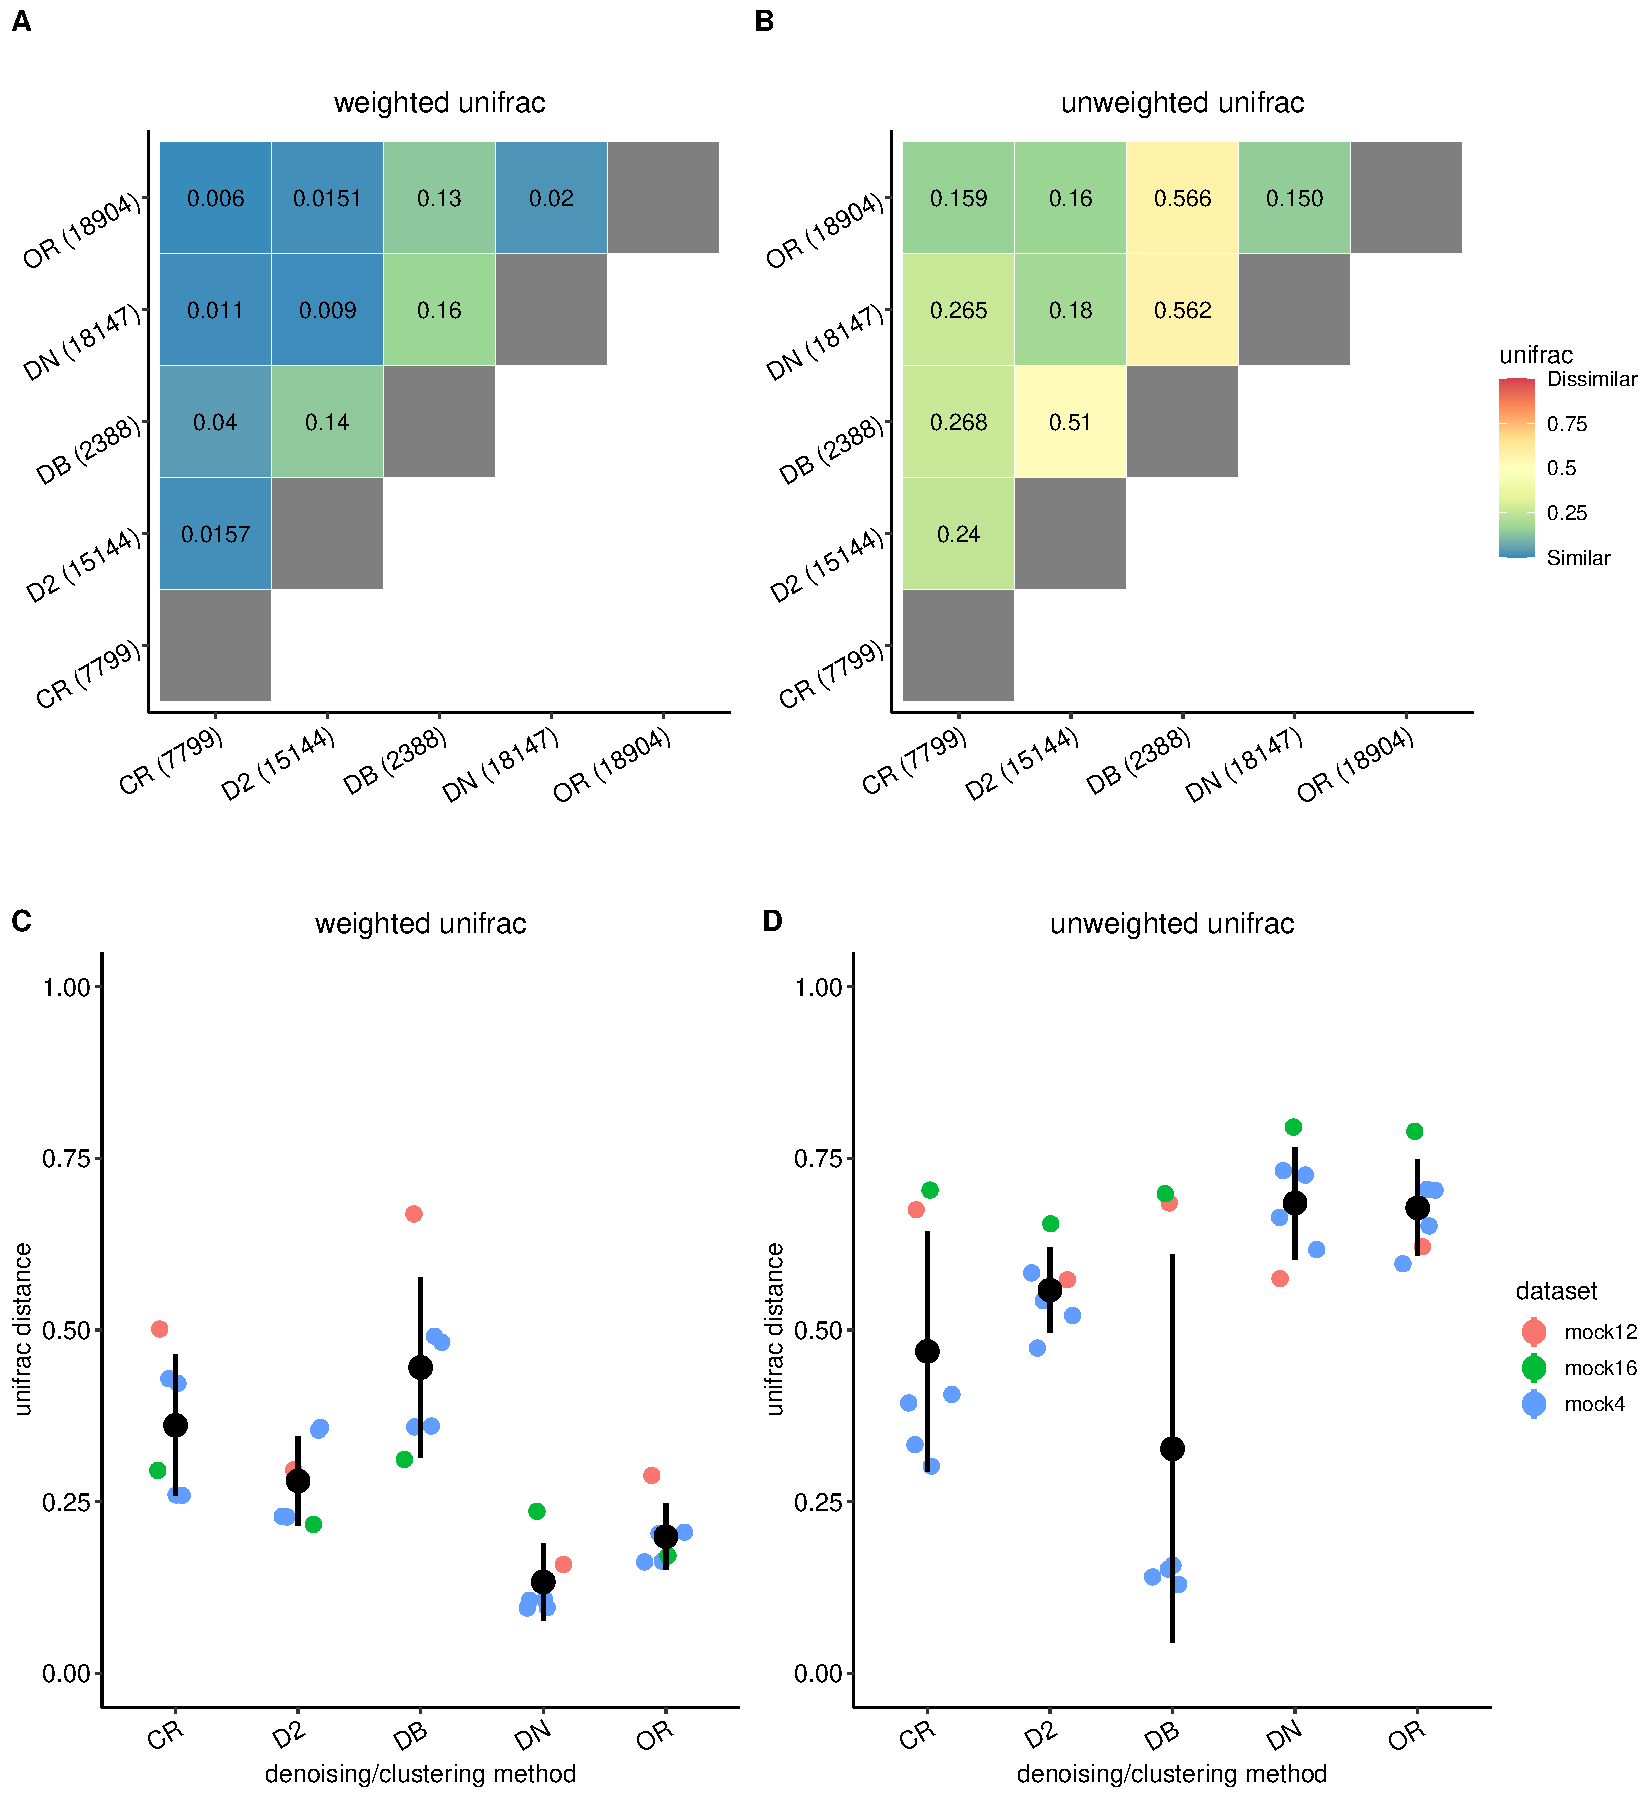
\includegraphics[width=\textwidth]{figure3.pdf}
  % \end{figure}
  \begin{figure}[H]
    \centering
    \caption{
      \textbf{Taxonomic reference databases vary in terms of their taxonomy assignments below the Order level}.
      \textbf{(A)} The taxonomic assignments of the top 50 representative sequences using the three different reference databases.
      This result illustrates how the same sequences are assigned to different genera under different databases.
      A significant portion of the representative sequences are assigned to an ``unknown'' Genus in two of three databases (\ac{gg} and \ac{ncbi}).
      The number of assigned genera for each database is displayed at the top of each column.
      \textbf{(B)} The number of representative sequences assigned to the same taxonomic label when using different reference databases (for the top 100 sequences).
      The mismatches are fewer at higher taxonomic levels, but, even at the Order level there exists greater than 51\% of mismatches, demonstrating the poor agreement in taxonomic labels assigned by the different databases.
      The data used for the analysis in (A, B) were samples (healthy and ASD) from the FMT dataset.
      \textbf{(C)} The Bray-Curtis dissimilarity between the predicted taxonomy profile and expected taxonomy profile in the mock datasets shows that there is no singular best choice of database for every dataset, as all the databases show similar performances.
      The \ac{gg} database and the Naive Bayes classifier are chosen as the defaults for the TA step of \ac{micone} due to their popularity.
      The datasets used for the analysis in (C) were the mock datasets from mockrobiota.
    }
    \label{fig:figure3}
  \end{figure}


  % \FloatBarrier
  % \newpage
  % \begin{figure}[H]
  %   \centering
  %   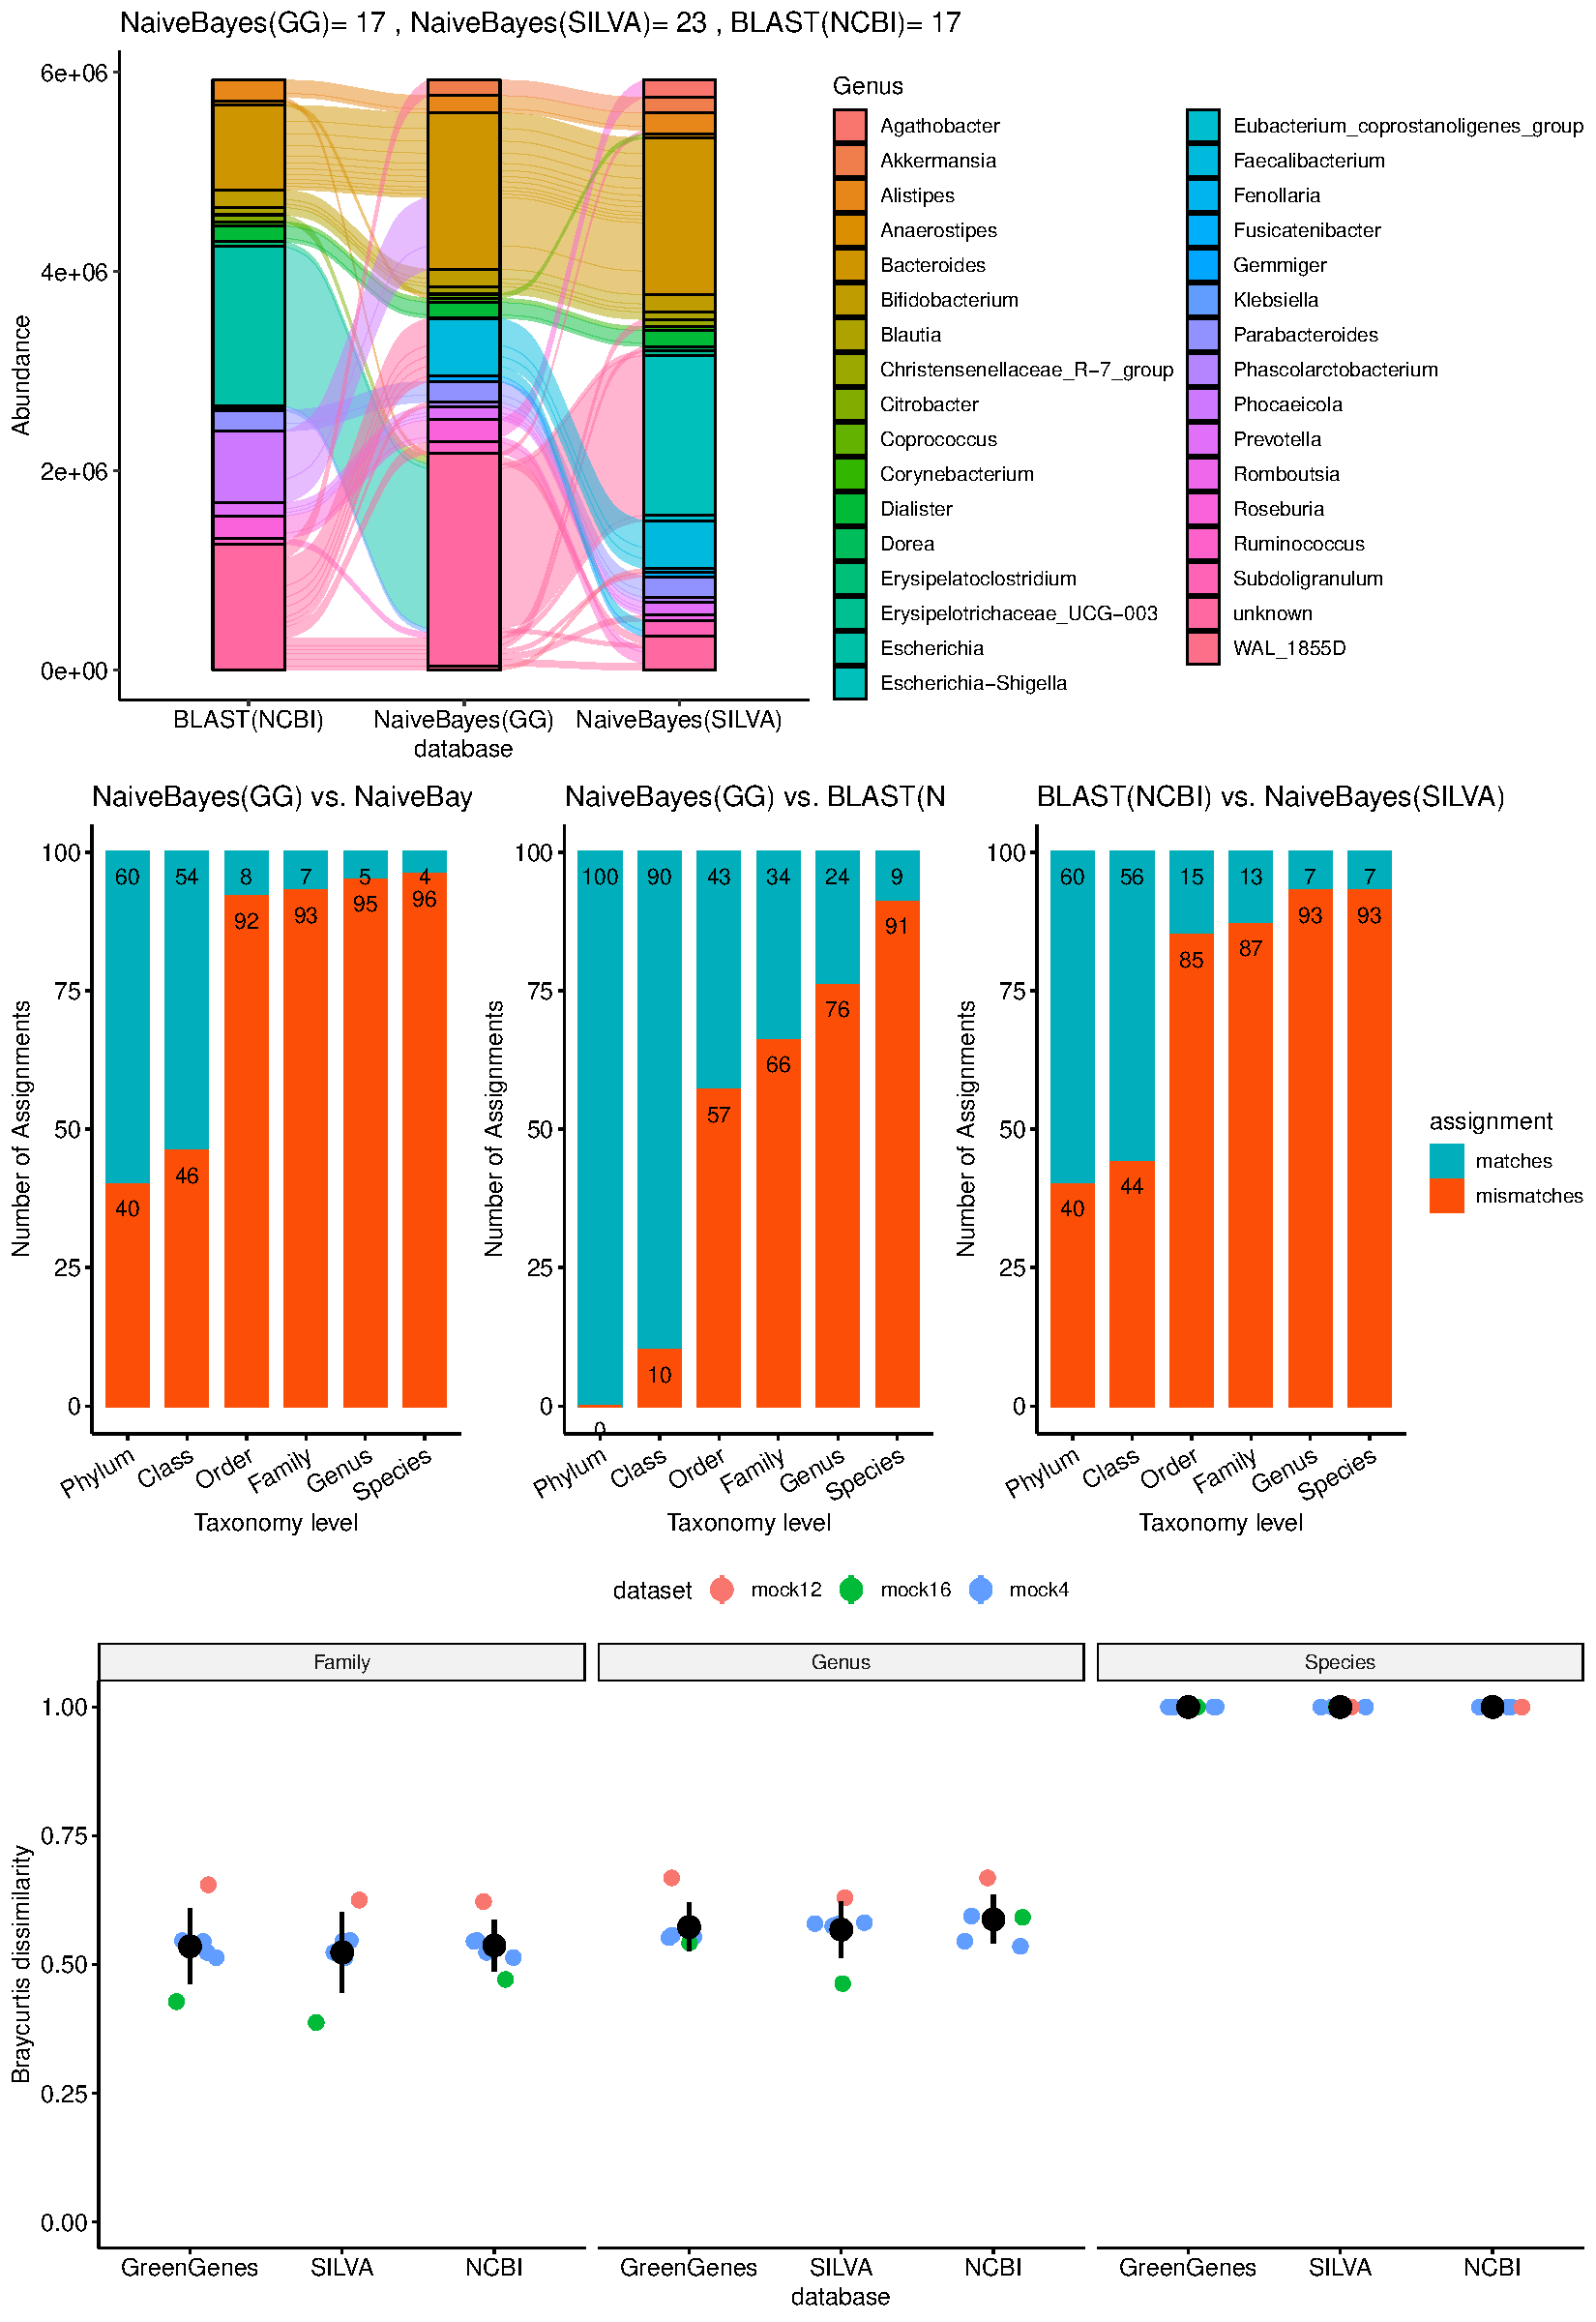
\includegraphics[width=\textwidth]{figure4.pdf}
  % \end{figure}
  \begin{figure}[H]
    \centering
    \caption{
      \textbf{Networks generated using different network inference methods show notable differences in terms of edge-density and connectivity}.
      \textbf{(A)} The nine different networks (excluding \acs{mldm}) generated by the different network inference methods.
      The nodes for each network (representing taxa) are arranged in the same positions in a circular layout and the differences in the connections can be directly visualized and compared.
      The green links are positive associations and the orange links represent negative associations.
      The networks look dissimilar and vary widely in terms of connectivity, and it is notable that the correlation-based methods generally produce networks with higher edge-densities.
      A threshold of 0.3 was set for the correlation-based methods (sparcc, propr, spearman and pearson) and a threshold of 0.01 was set for the direct association methods (flashweave, spieceasi, cozine, harmonies, and spring).
      \textbf{(B)} The node overlap Upset plot indicates that all the networks have a large proportion of common nodes involved in connections (33 out of 68).
      Conversely \textbf{(C)}, the edge overlap Upset plot shows that a very small fraction of these connections are actually shared (8 out of 202).
      The data used in this analysis were the healthy stool samples from the FMT dataset.
      \acs{mldm} is not shown in the comparisons because the algorithm failed to converge for the particular network combination used here (default setting of the \ac{micone} pipeline).
    }
    \label{fig:figure4}
  \end{figure}


  % \FloatBarrier
  % \newpage
  % \begin{figure}[H]
  %   \centering
  %   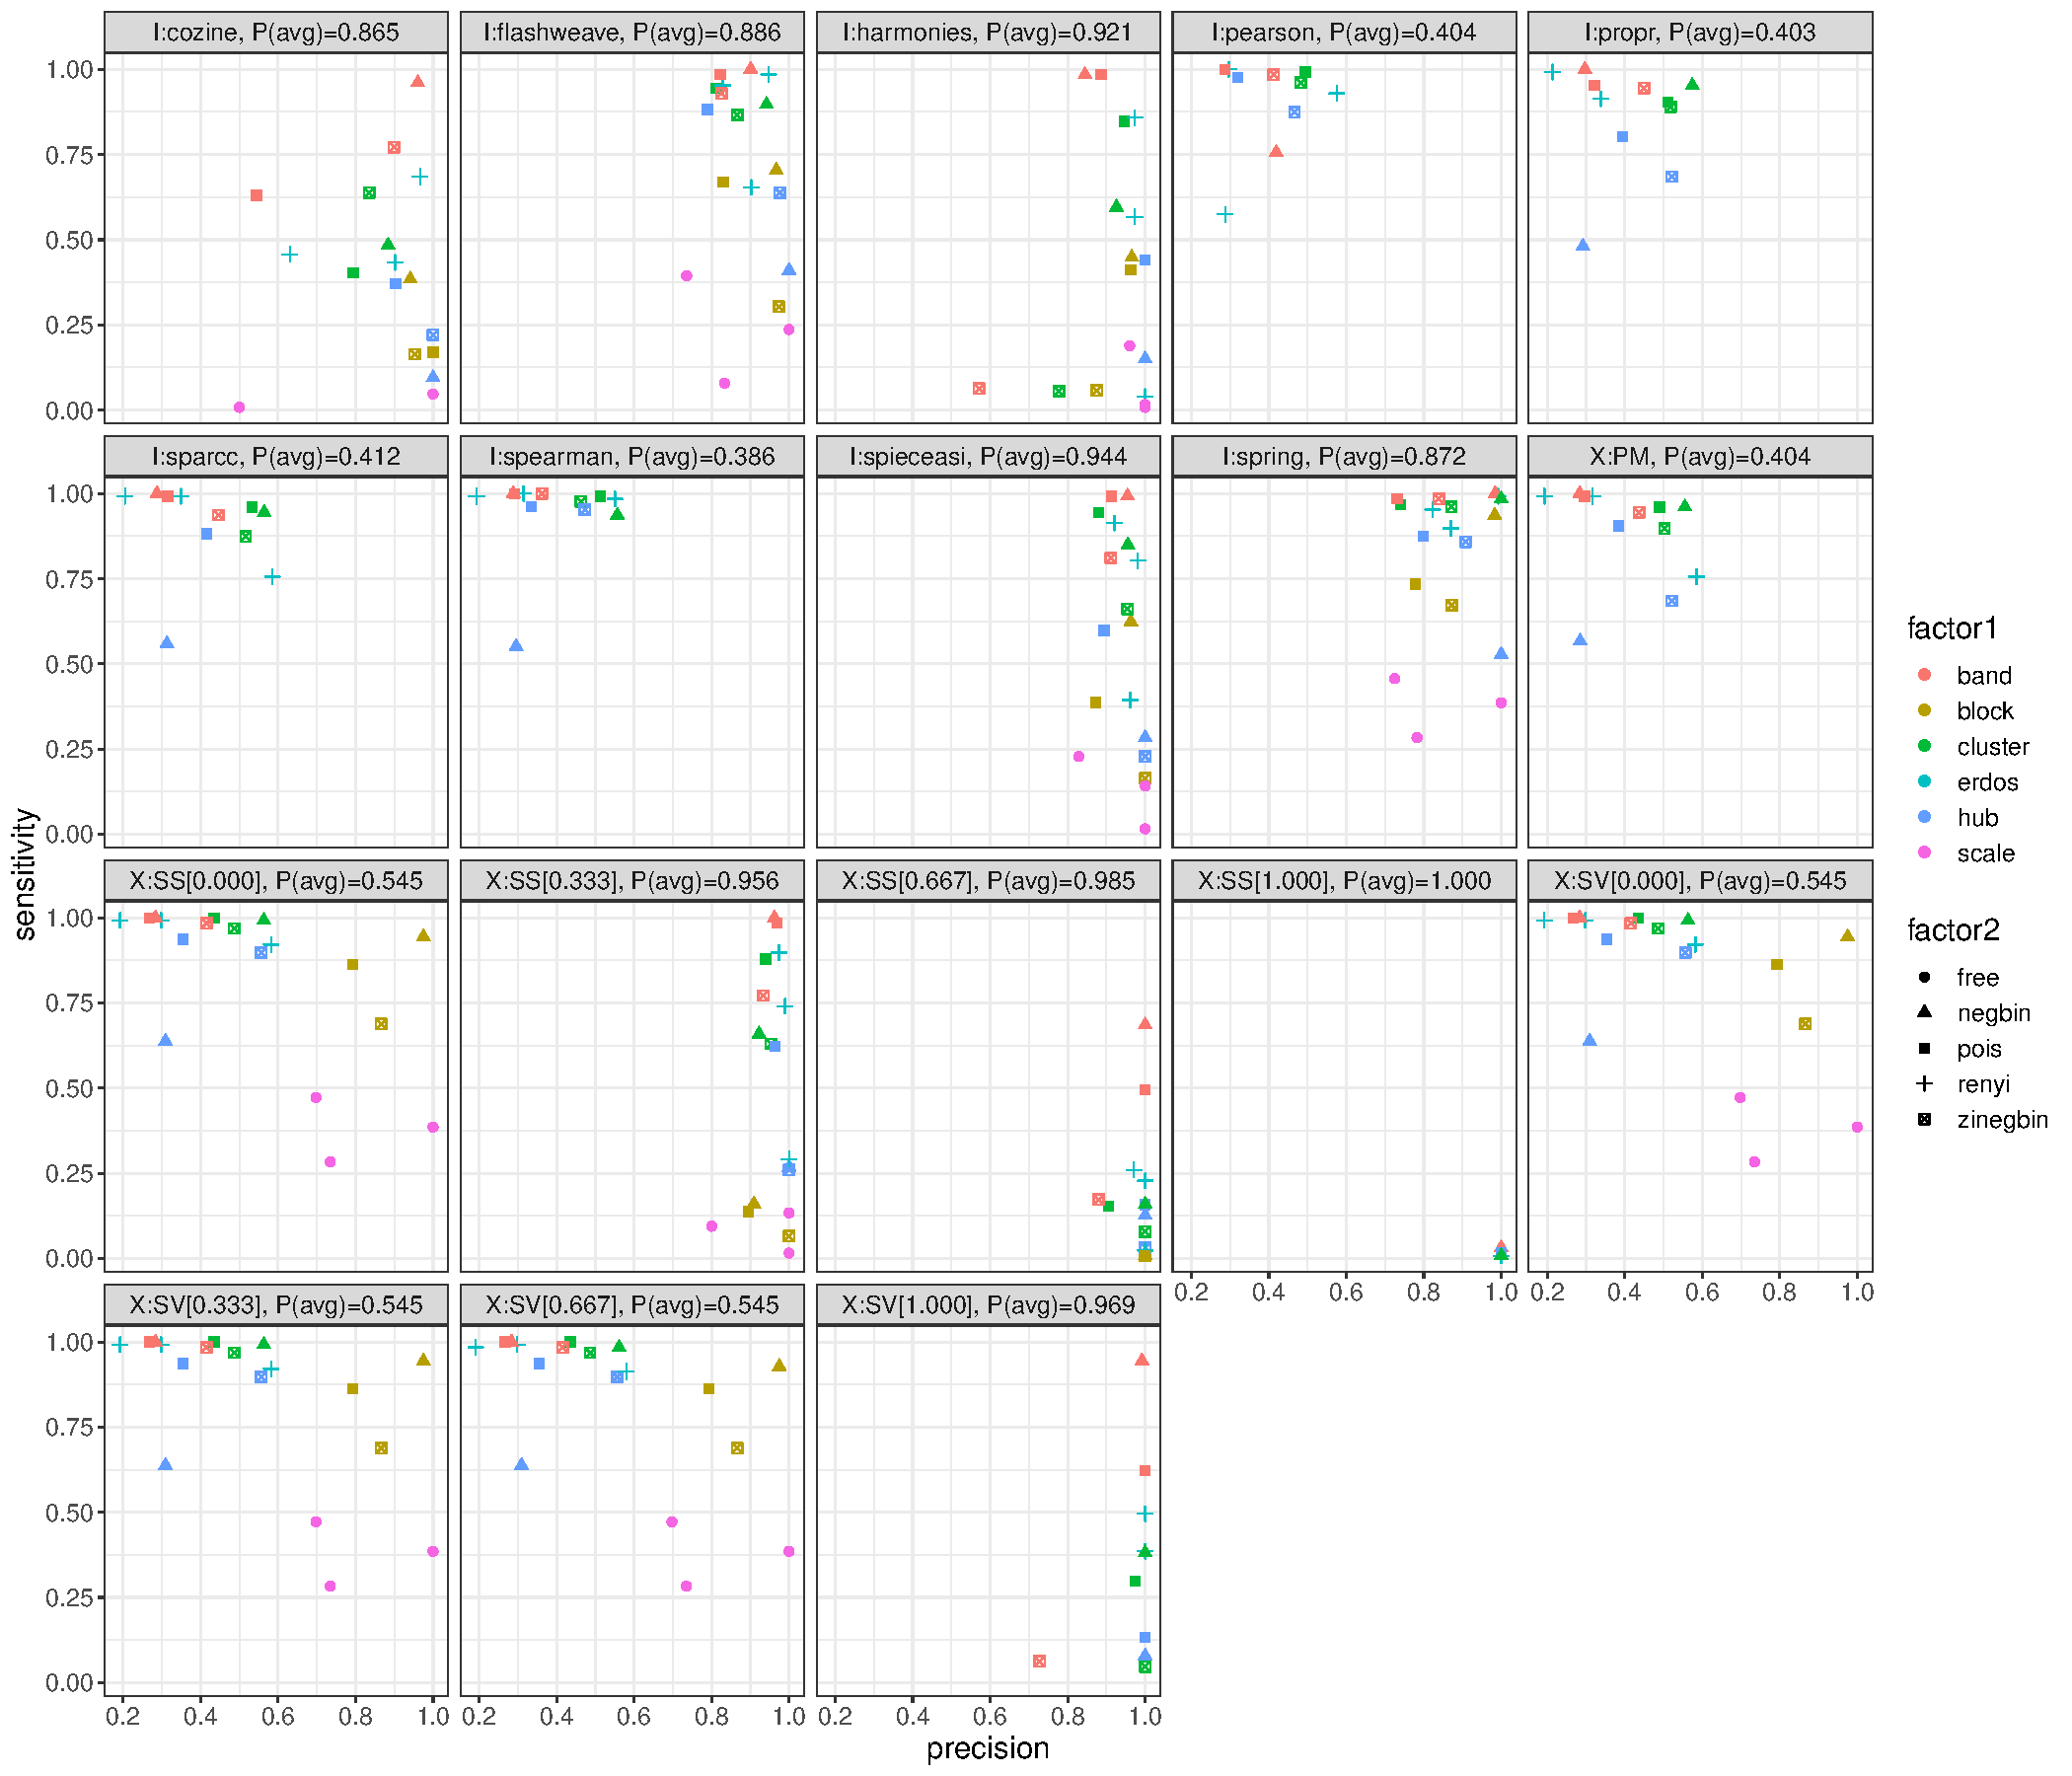
\includegraphics[width=1.0\linewidth]{figure5.pdf}
  % \end{figure}
  \begin{figure}[H]
    \centering
    \caption{
      \textbf{The associations generated by the scaled-sum consensus method show high precision in benchmarks using synthetic datasets}.
    The different points on the box plot show the precision of co-occurrence networks generated through individual network inference methods and through consensus network construction approaches. Precision is estimated based on the comparisons with two sets of synthetic benchmark datasets (``NorTA'' and ``seqtime'', see Methods).
      The independent algorithms chosen for the comparison are the two best-performing correlation-based (propr, sparcc) and direct association based (spieceasi, flashweave) methods.
      For consensus network inference, we used the scaled-sum (SS) and simple voting (SV) methods.
      A weight threshold of 0.1 and a p-value threshold of 0.05 was applied to each network before the calculation of precision.
      The overall best precision was consistently obtained by the scaled-sum consensus method for $p \geq 0.333$ on both benchmark datasets. Among all the individual network inference methods, spieceasi shows the best average precision.
      The simple voting method, when using the presence of edges in all inferred networks as a requirement ($p = 1.000$), also outperforms spieceasi on average precision.
      Therefore, we set the scaled-sum consensus method with $p = 0.333$ as the default tool for consensus network inference, since this option provides a good balance of precision and sensitivity (see also Figure~\ref{fig:figure_s5} and \ref{fig:figure_s6}).
    }
    \label{fig:figure5}
  \end{figure}


  % \FloatBarrier
  % \newpage
  % \begin{figure}[H]
  %   \centering
  %   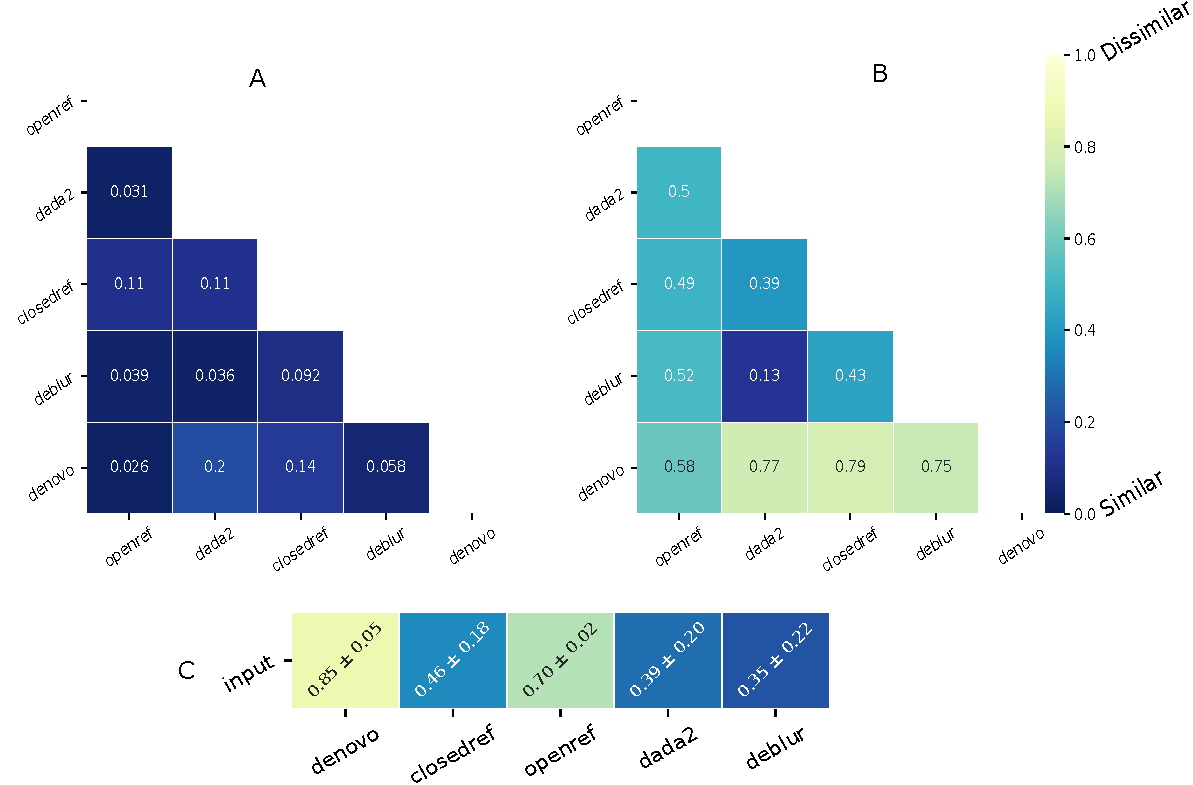
\includegraphics[width=\textwidth]{figure6.pdf}
  % \end{figure}
  \begin{figure}[H]
    \centering
      \caption{
      \textbf{The choice of reference database has the largest impact on network variance}.
      \textbf{(A)} The percentage of variance in the networks (from the  FMT dataset) contributed by the \acf{dc}, CC (chimera checking), \acf{ta}, \acf{op} and \acf{ni} steps of the pipeline calculated using ANOVA on a linear model (see Methods).
      A weight threshold of 0.1 and a p-value threshold of 0.05 were applied to each network before the analysis.
      The taxonomy database contributes most to the variance between the networks (65.4\%) followed by the filtering of the counts matrix (26.8\%) in the OP step.
    The variation due to the NI, DC and CC steps are much smaller in comparison (6.553\%, 0.648\%, and 0.003\% respectively).
      The negligible fraction labeled as the residual is an artifact that arises when multiple steps are changed at the same time.
      \textbf{(B)} All the inferred networks generated from various combinations of tools are shown as points on a PCA plot.
      Each point on the PCA plot represents a network inferred using different combinations of tools and parameters that are available in the \ac{micone} pipeline.
      The color of the points corresponds to the tools used at each step of the pipeline (DC, TA, OP, and NI).
      The points on the PCA plot can be grouped based on the TA step, but the extent of this separation decreases when the filtering is turned on in the OP step, confirming that the variability in the networks decreased upon filtering out the taxonomic entities at low abundance.
      Some algorithms, especially the direct association methods, at the NI step can also be seen to generate networks that are less variable compared to the others.
      The \ac{dc} step does not seem to have any correlation with the variation in the networks on the PCA plot.
    }
    \label{fig:figure6}
  \end{figure}


  % \FloatBarrier
  % \newpage
  % \begin{figure}[H]
  %   \centering
  %   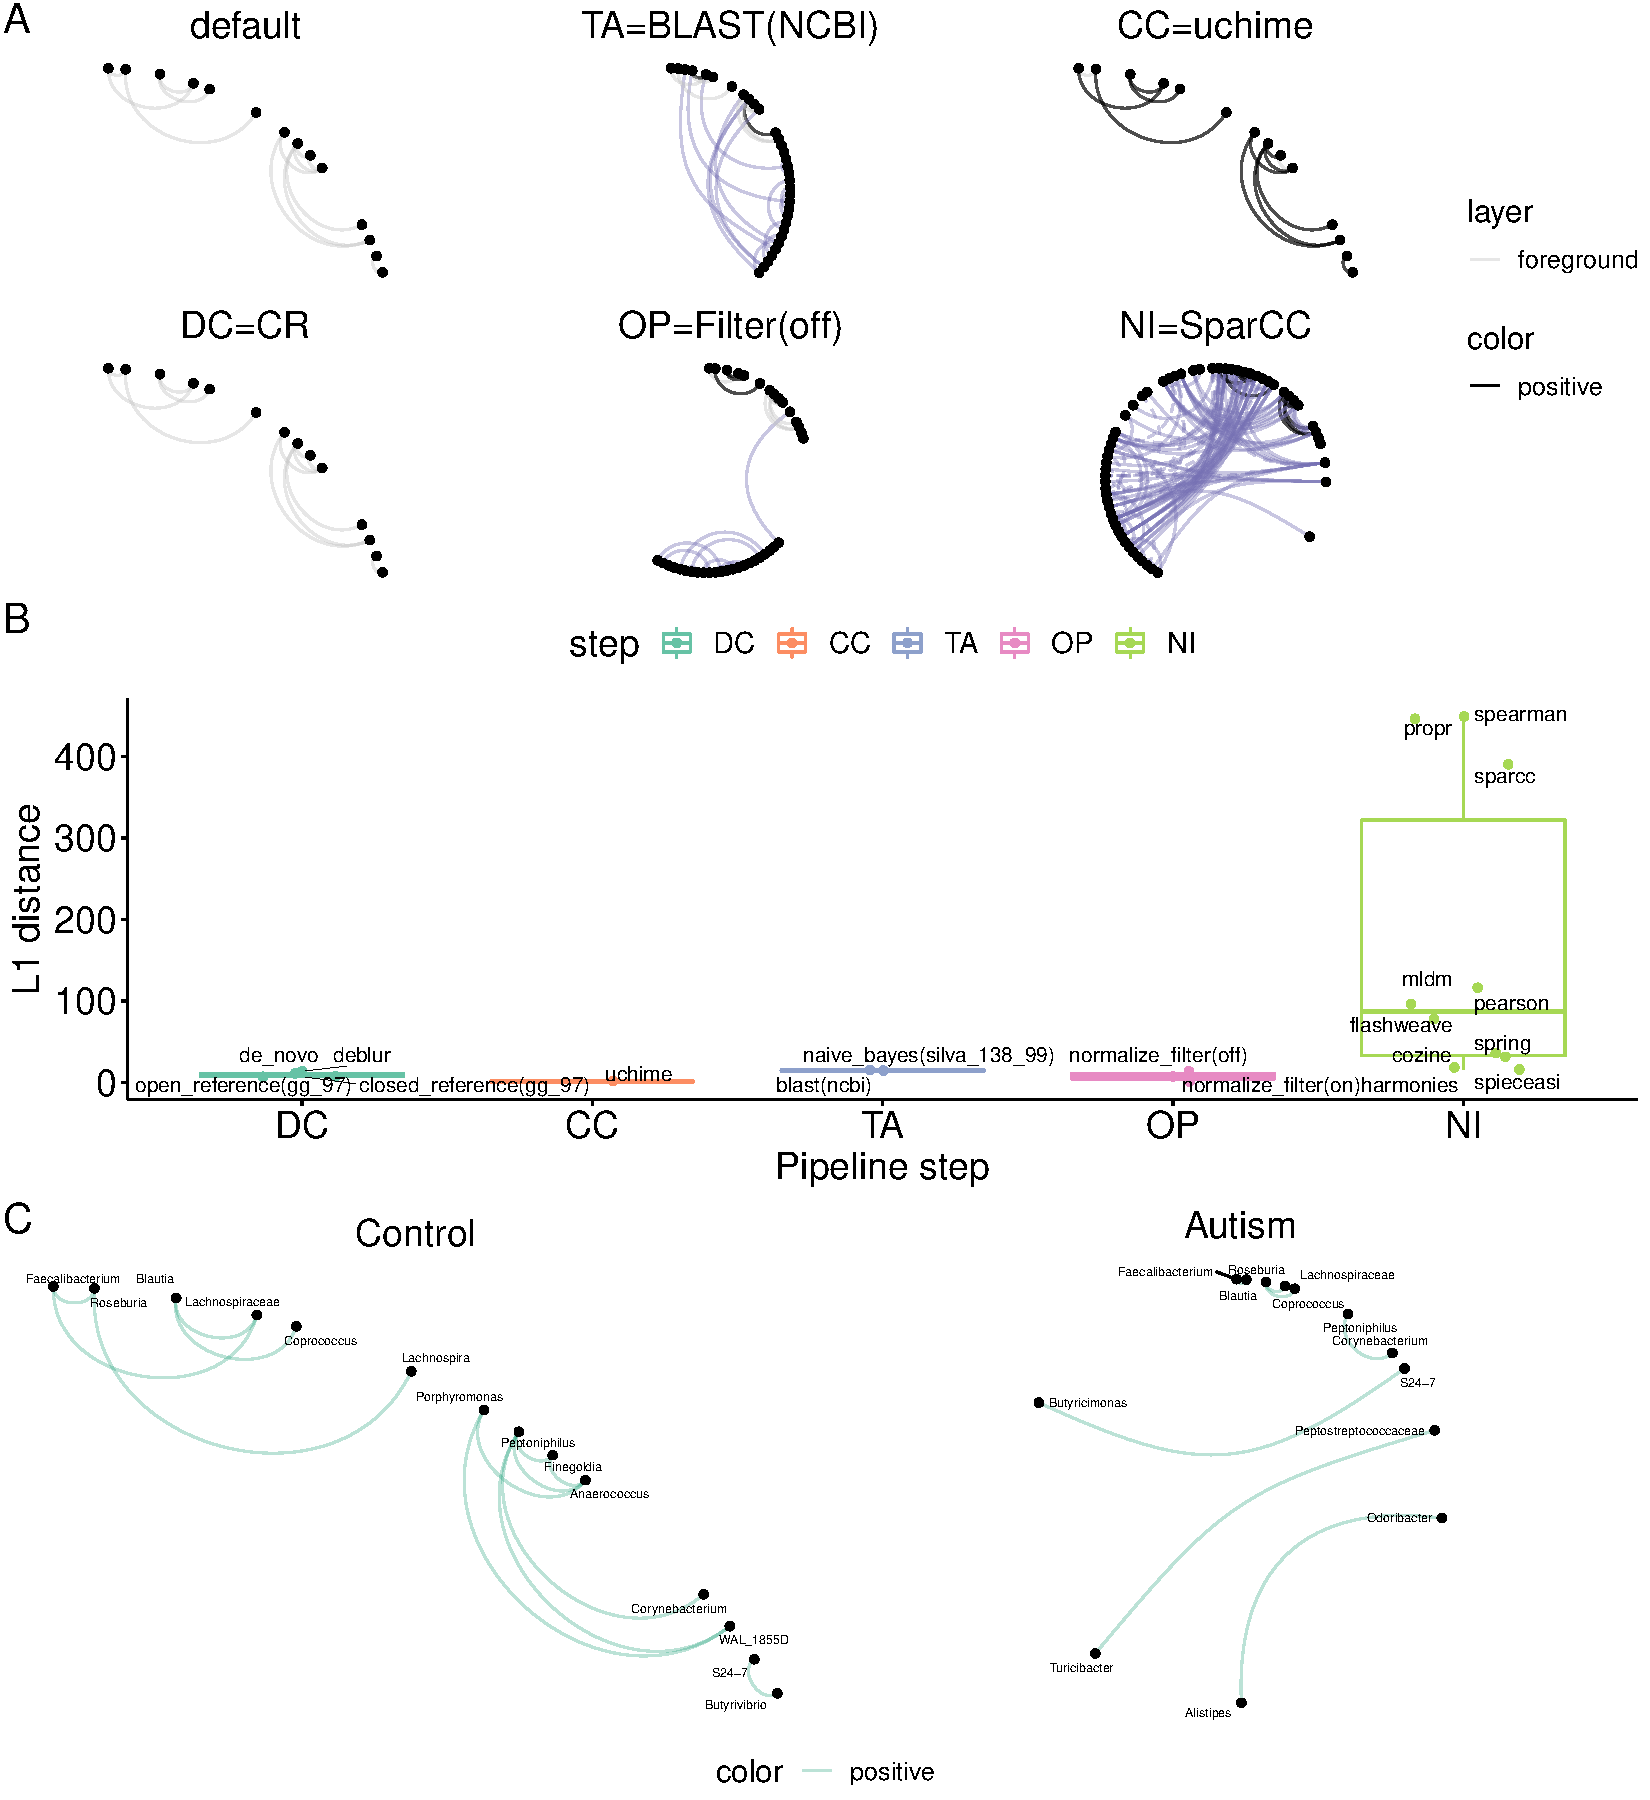
\includegraphics[width=1.0\linewidth]{figure7.pdf}
  % \end{figure}
  \begin{figure}[H]
    \centering
    \caption{
      \textbf{Comparison of networks generated from the control and ASD samples of the FMT dataset using the \ac{micone} pipeline}.
      The networks for the control (left) and ASD (right) samples were generated using the default tools and parameters recommended by the \ac{micone} pipeline as described in Table~\ref{tab:micone_tools}.
      There are 22 unique links in the network for control samples, 12 unique links in the network for ASD subjects, and 7 edges in common between both networks.
      The changes in these connections can serve as potential starting points for further experimental validations or literature surveys.
    }
    \label{fig:figure7}
  \end{figure}


  \FloatBarrier
  \newpage
  \subsection*{Supplementary Tables and Figures}

  \renewcommand{\thefigure}{S\arabic{figure}}
  \setcounter{figure}{0}

  \renewcommand{\thetable}{S\arabic{table}}
  \setcounter{table}{0}

  \begin{table}[H]
    \centering
    \caption{
      \textbf{Table of global network metrics for networks inferred from all possible combinations of tools}.
      In each row, one tool in a particular step is kept constant, and the metric is calculated for every possible combination of tools for the other steps of the pipeline.
      Therefore, each row shows the grouped average metric for each tool in every step of the pipeline.
      The network inference methods show the most variation in the global network metrics compared to tools in other steps of the pipeline.
    }
    \label{tab:network_metrics}
  \end{table}


    % \begin{figure}[H]
    %   \centering
    %   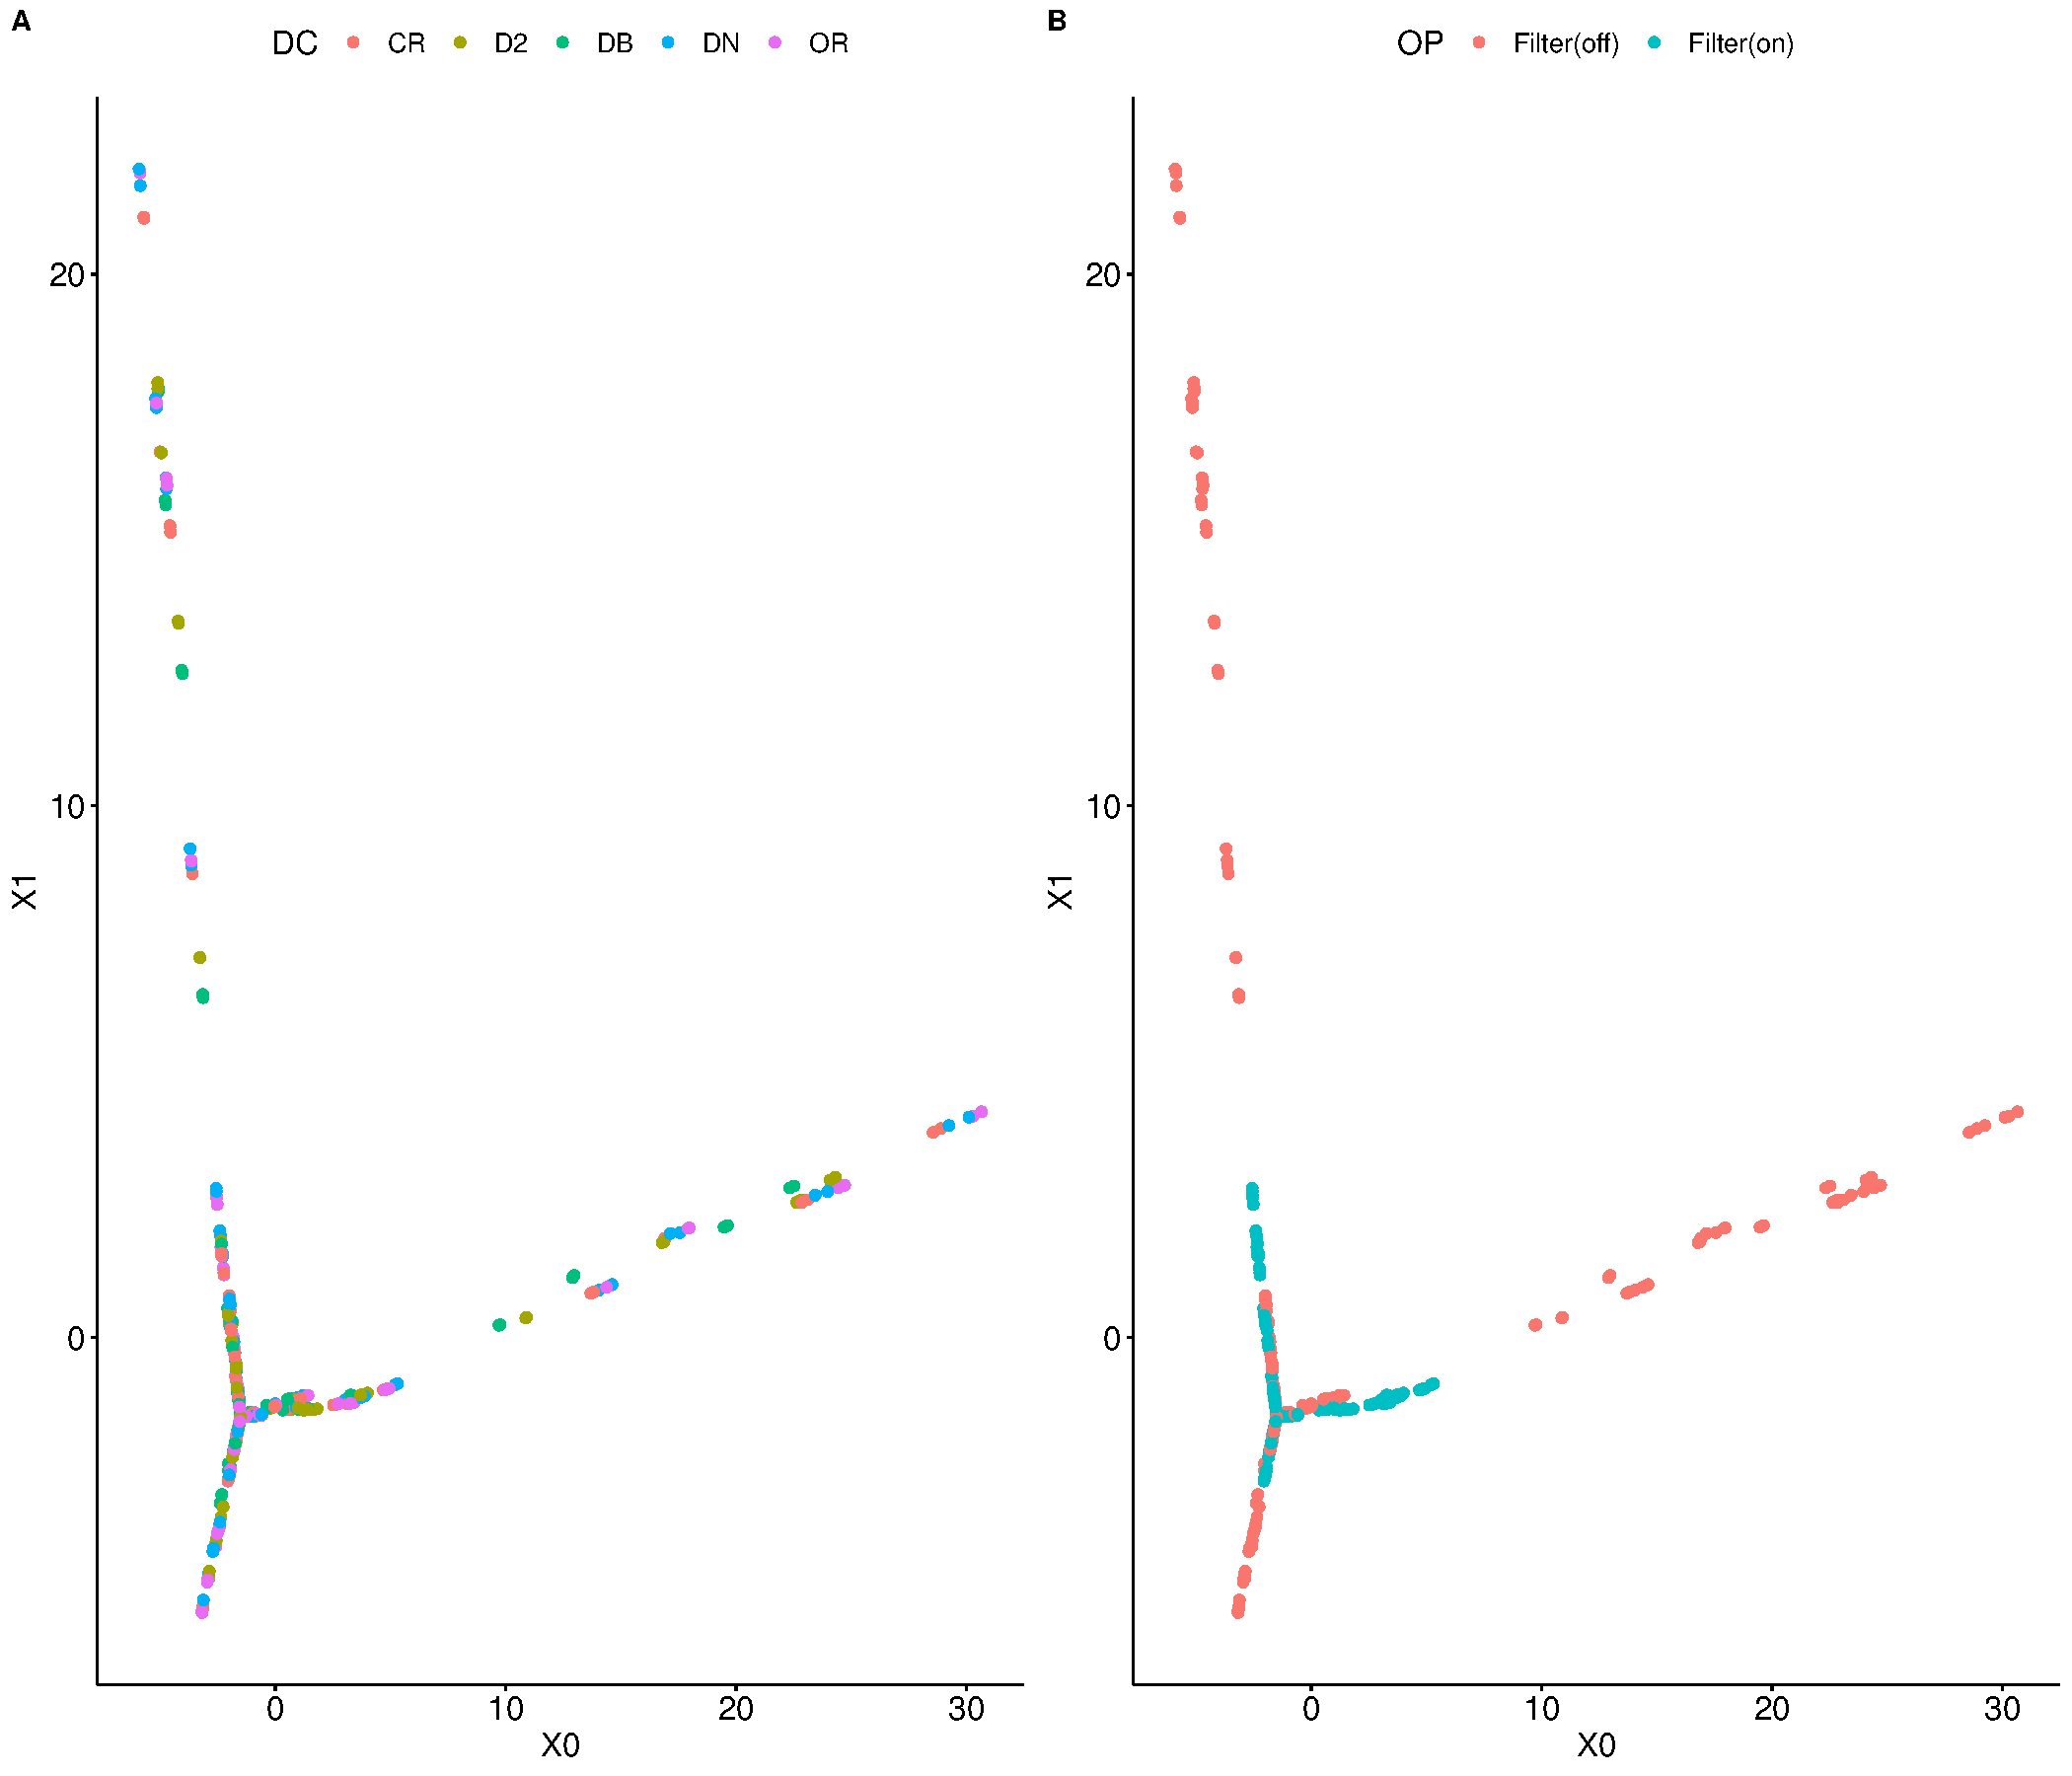
\includegraphics[width=1.0\linewidth]{figure_s1.pdf}
    % \end{figure}
    \begin{figure}[H]
      \centering
        \caption{
          \textbf{The t-SNE plot of all the inferred networks clusters the networks based on the taxonomy reference database used}.
          Each point on the t-SNE plot represents a network inferred using different combinations of tools and parameters that are available in the \ac{micone} pipeline.
          The points are colored by the tools and parameters used in \ac{dc} step (A), \ac{ta} step (B), \ac{op} step (C) and \ac{ni} step (D).
          The separation of the points based on taxonomy reference database shows that the points cluster based on reference database in high-dimensional space.
        }
      \label{fig:figure_s1}
    \end{figure}
    % \FloatBarrier
    % \newpage

    % \begin{figure}[H]
    %   \centering
    %   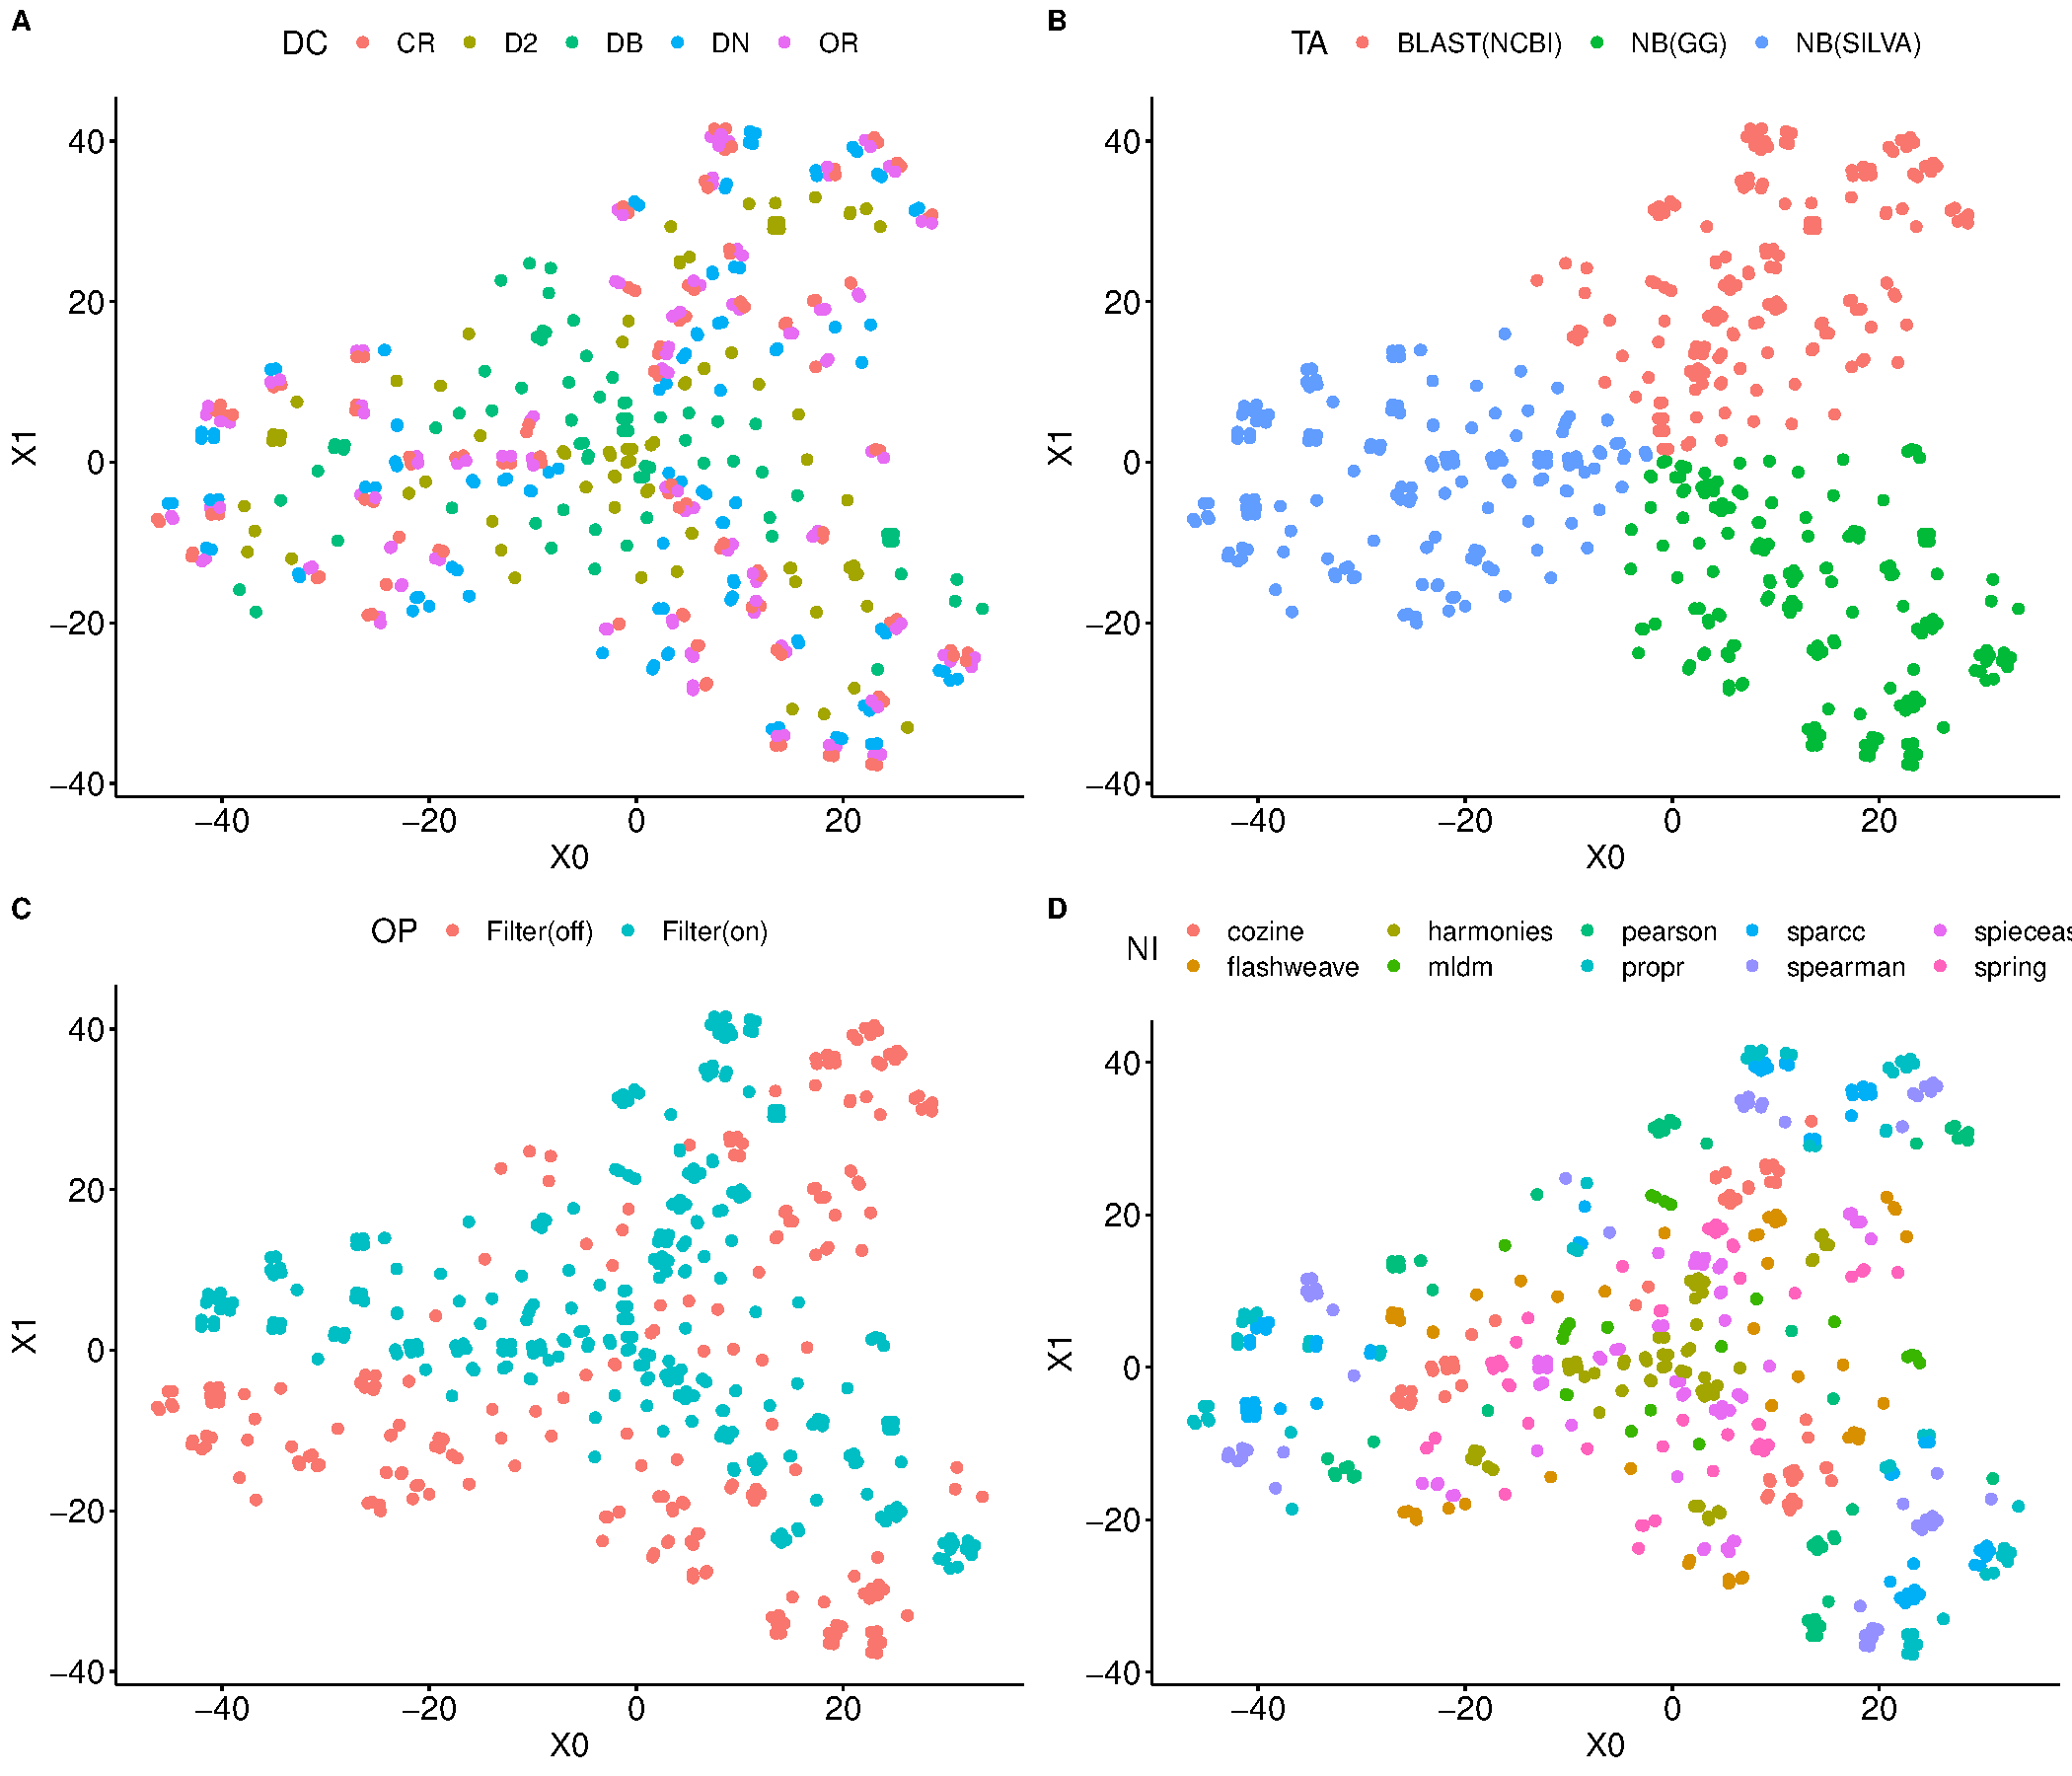
\includegraphics[width=1.0\linewidth]{figure_s2.pdf}
    % \end{figure}
    \begin{figure}[H]
      \centering
        \caption{
          \textbf{The UniFrac distance between the 1000 most abundant representative sequences is higher than that when all sequences are considered}.
          Each value is the average UniFrac distance between the reference sequences generated by the various methods in the \ac{dc} step (similar to Figure~\ref{fig:figure2}).
          There is an increase in both weighted and unweighted UniFrac distances compared to when all the representative sequences are considered.
          This shows that the 1000 most abundant representative sequences generated by the DC methods are not as similar to each other.
          And since the weighted UniFrac is much smaller than the unweighted UniFrac distance, we can conclude that those reference sequences that are present in the middle of the abundance distribution (considering all sequences) are dissimilar.
        }
      \label{fig:figure_s2}
    \end{figure}
    % \FloatBarrier
    % \newpage

    % \begin{figure}[H]
    %   \centering
    %   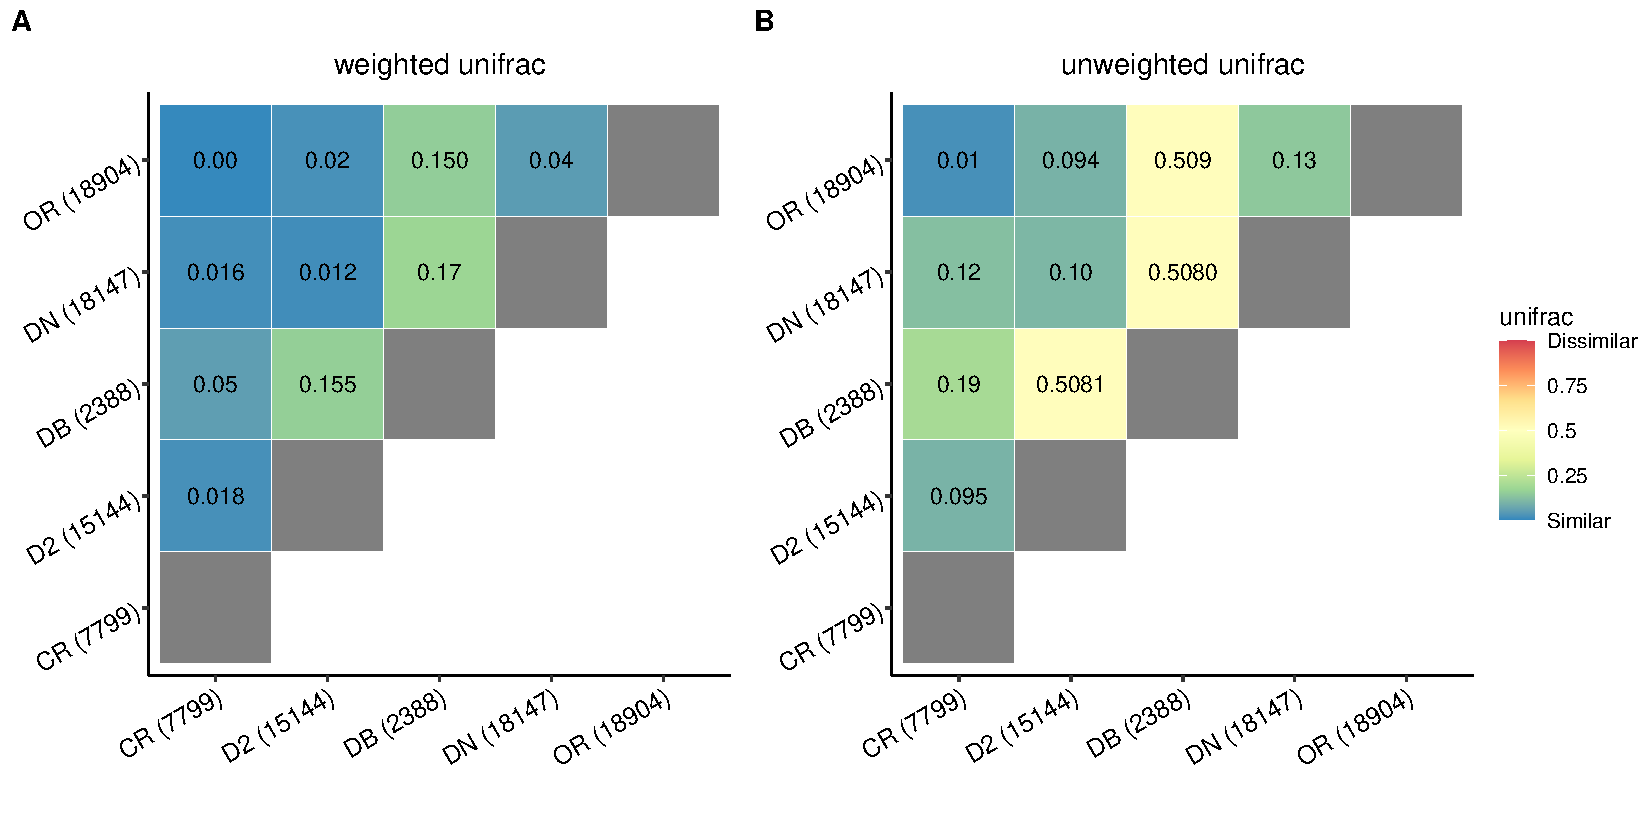
\includegraphics[width=1.0\linewidth]{figure_s3.pdf}
    % \end{figure}
    \begin{figure}[H]
      \centering
        \caption{
          \textbf{The weighted and unweighted UniFrac distances are small for the representative sequences generated using remove bimera and uchime for each denoising method}.
          With the exception of de novo and open reference under the unweighted UniFrac metric, all the other methods have high similarity, implying that the two chimera checking methods, uchime and remove bimera, produce similar outputs.
          This is especially true for the \ac{dada2} and Deblur methods which are the recommended denoising methods in the \ac{micone} pipeline.
          Therefore, remove bimera is recommended as the default chimera method if one is using \ac{dada2} and uchime-denovo when one is using Deblur, since these methods were developed for these respective algorithms (\ac{qiime2} uses uchime-denovo in the Deblur workflow).
        }
      \label{fig:figure_s3}
    \end{figure}
    % \FloatBarrier
    % \newpage

    % \begin{figure}[H]
    %   \centering
    %   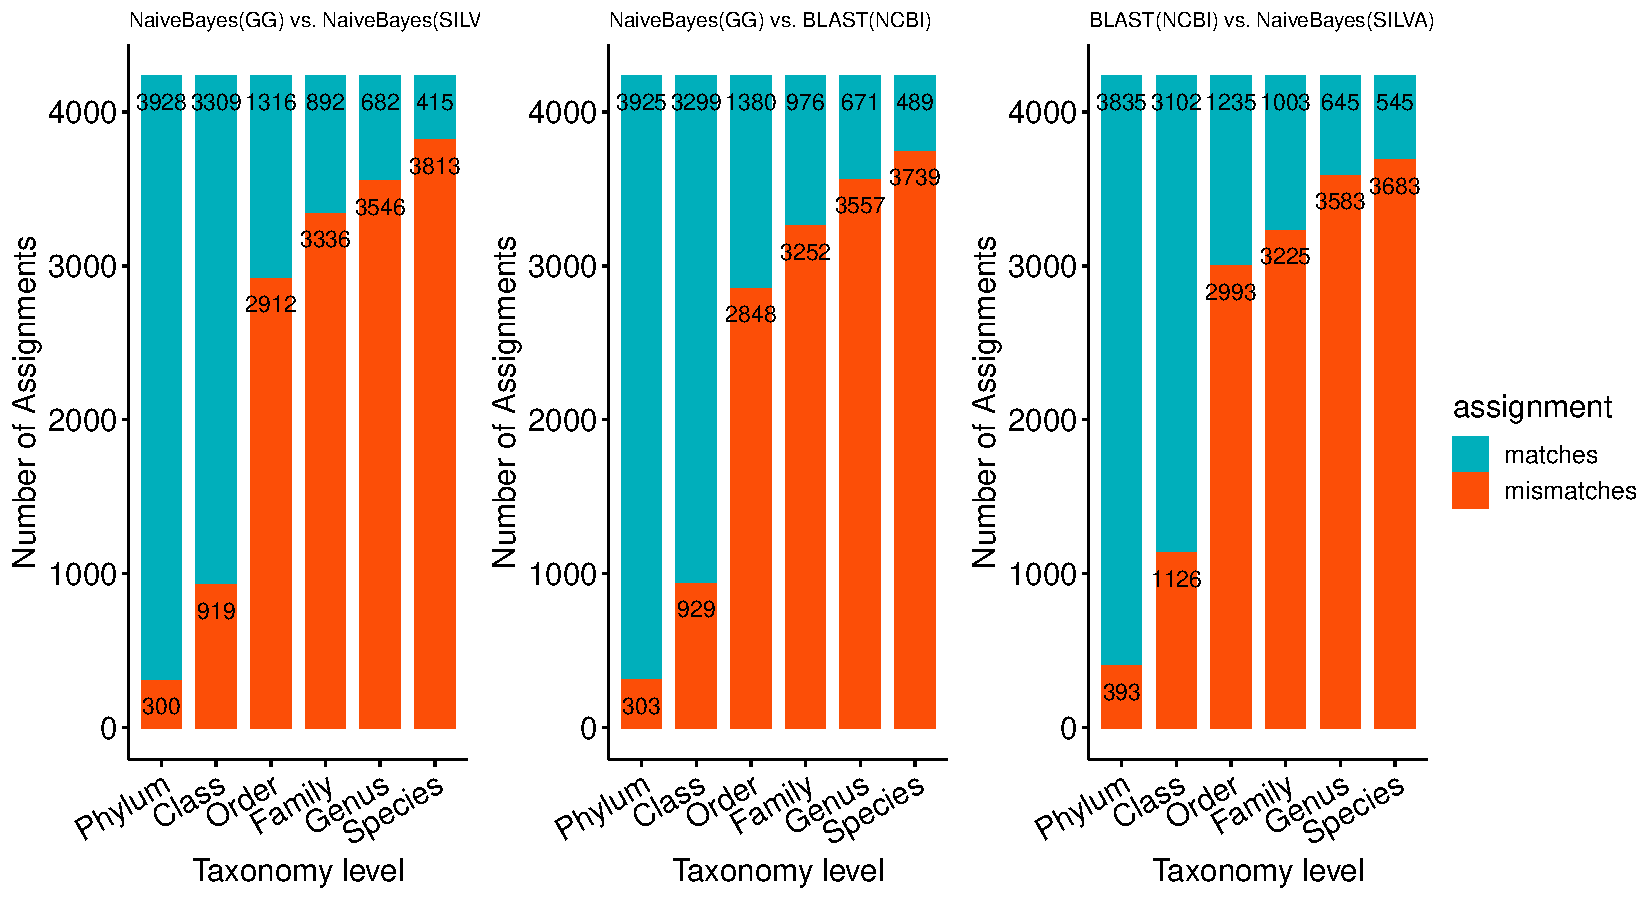
\includegraphics[width=1.0\linewidth]{figure_s4.pdf}
    % \end{figure}
    \begin{figure}[H]
      \centering
        \caption{
          \textbf{The pairwise comparison of assignments generated using different databases for all representative sequences has a higher proportion of mismatches}.
          The comparison made here is similar to Figure~\ref{fig:figure3}B, but instead of the top 100 taxonomic entities (by abundance), all the assignments from one database are matched with those from the other two databases.
          The higher percentage of mismatches implies that the assigned taxonomies in the more abundant sequences (top 100) match more consistently.
        }
      \label{fig:figure_s4}
    \end{figure}
    % \FloatBarrier
    % \newpage

  % \begin{figure}[H]
  %   \centering
  %   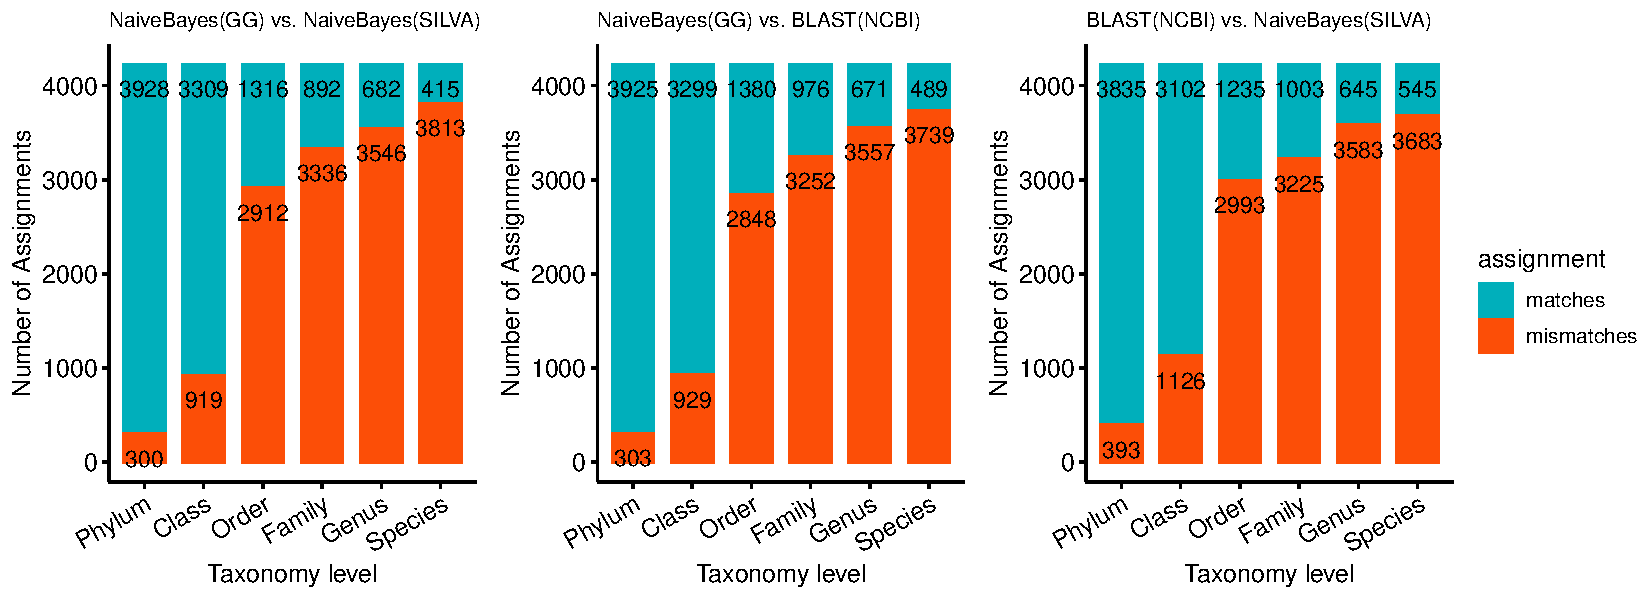
\includegraphics[width=1.0\linewidth]{figure_s5.pdf}
  % \end{figure}
  \begin{figure}[H]
    \centering
      \caption{
        \textbf{The precision and sensitivity of the inferred networks on the ``NorTA'' synthetic interaction data}.
        The different consensus methods used are scaled-sum (SS) and simple voting (SV) methods.
        Pearson and Spearman methods are not used in the calculation of the consensus.
        Among all the independent network inference methods, \acs{spieceasi} has the best average precision (0.944), but the overall best precision was consistently obtained by the scaled-sum method (0.956, 0.985, and 1.000).
        The simple voting method when using the presence of edges in all inferred networks as a requirement ($p = 1.000$), also outperforms \acs{spieceasi} on average precision (0.969).
        Although \acs{spieceasi} has a higher sensitivity, if the goal of network inference is to obtain the list of associations that have a high probability of existing in the real microbial community, then the consensus methods perform better.
      }
    \label{fig:figure_s5}
  \end{figure}
  % \FloatBarrier
  % \newpage

  % \begin{figure}[H]
  %   \centering
  %   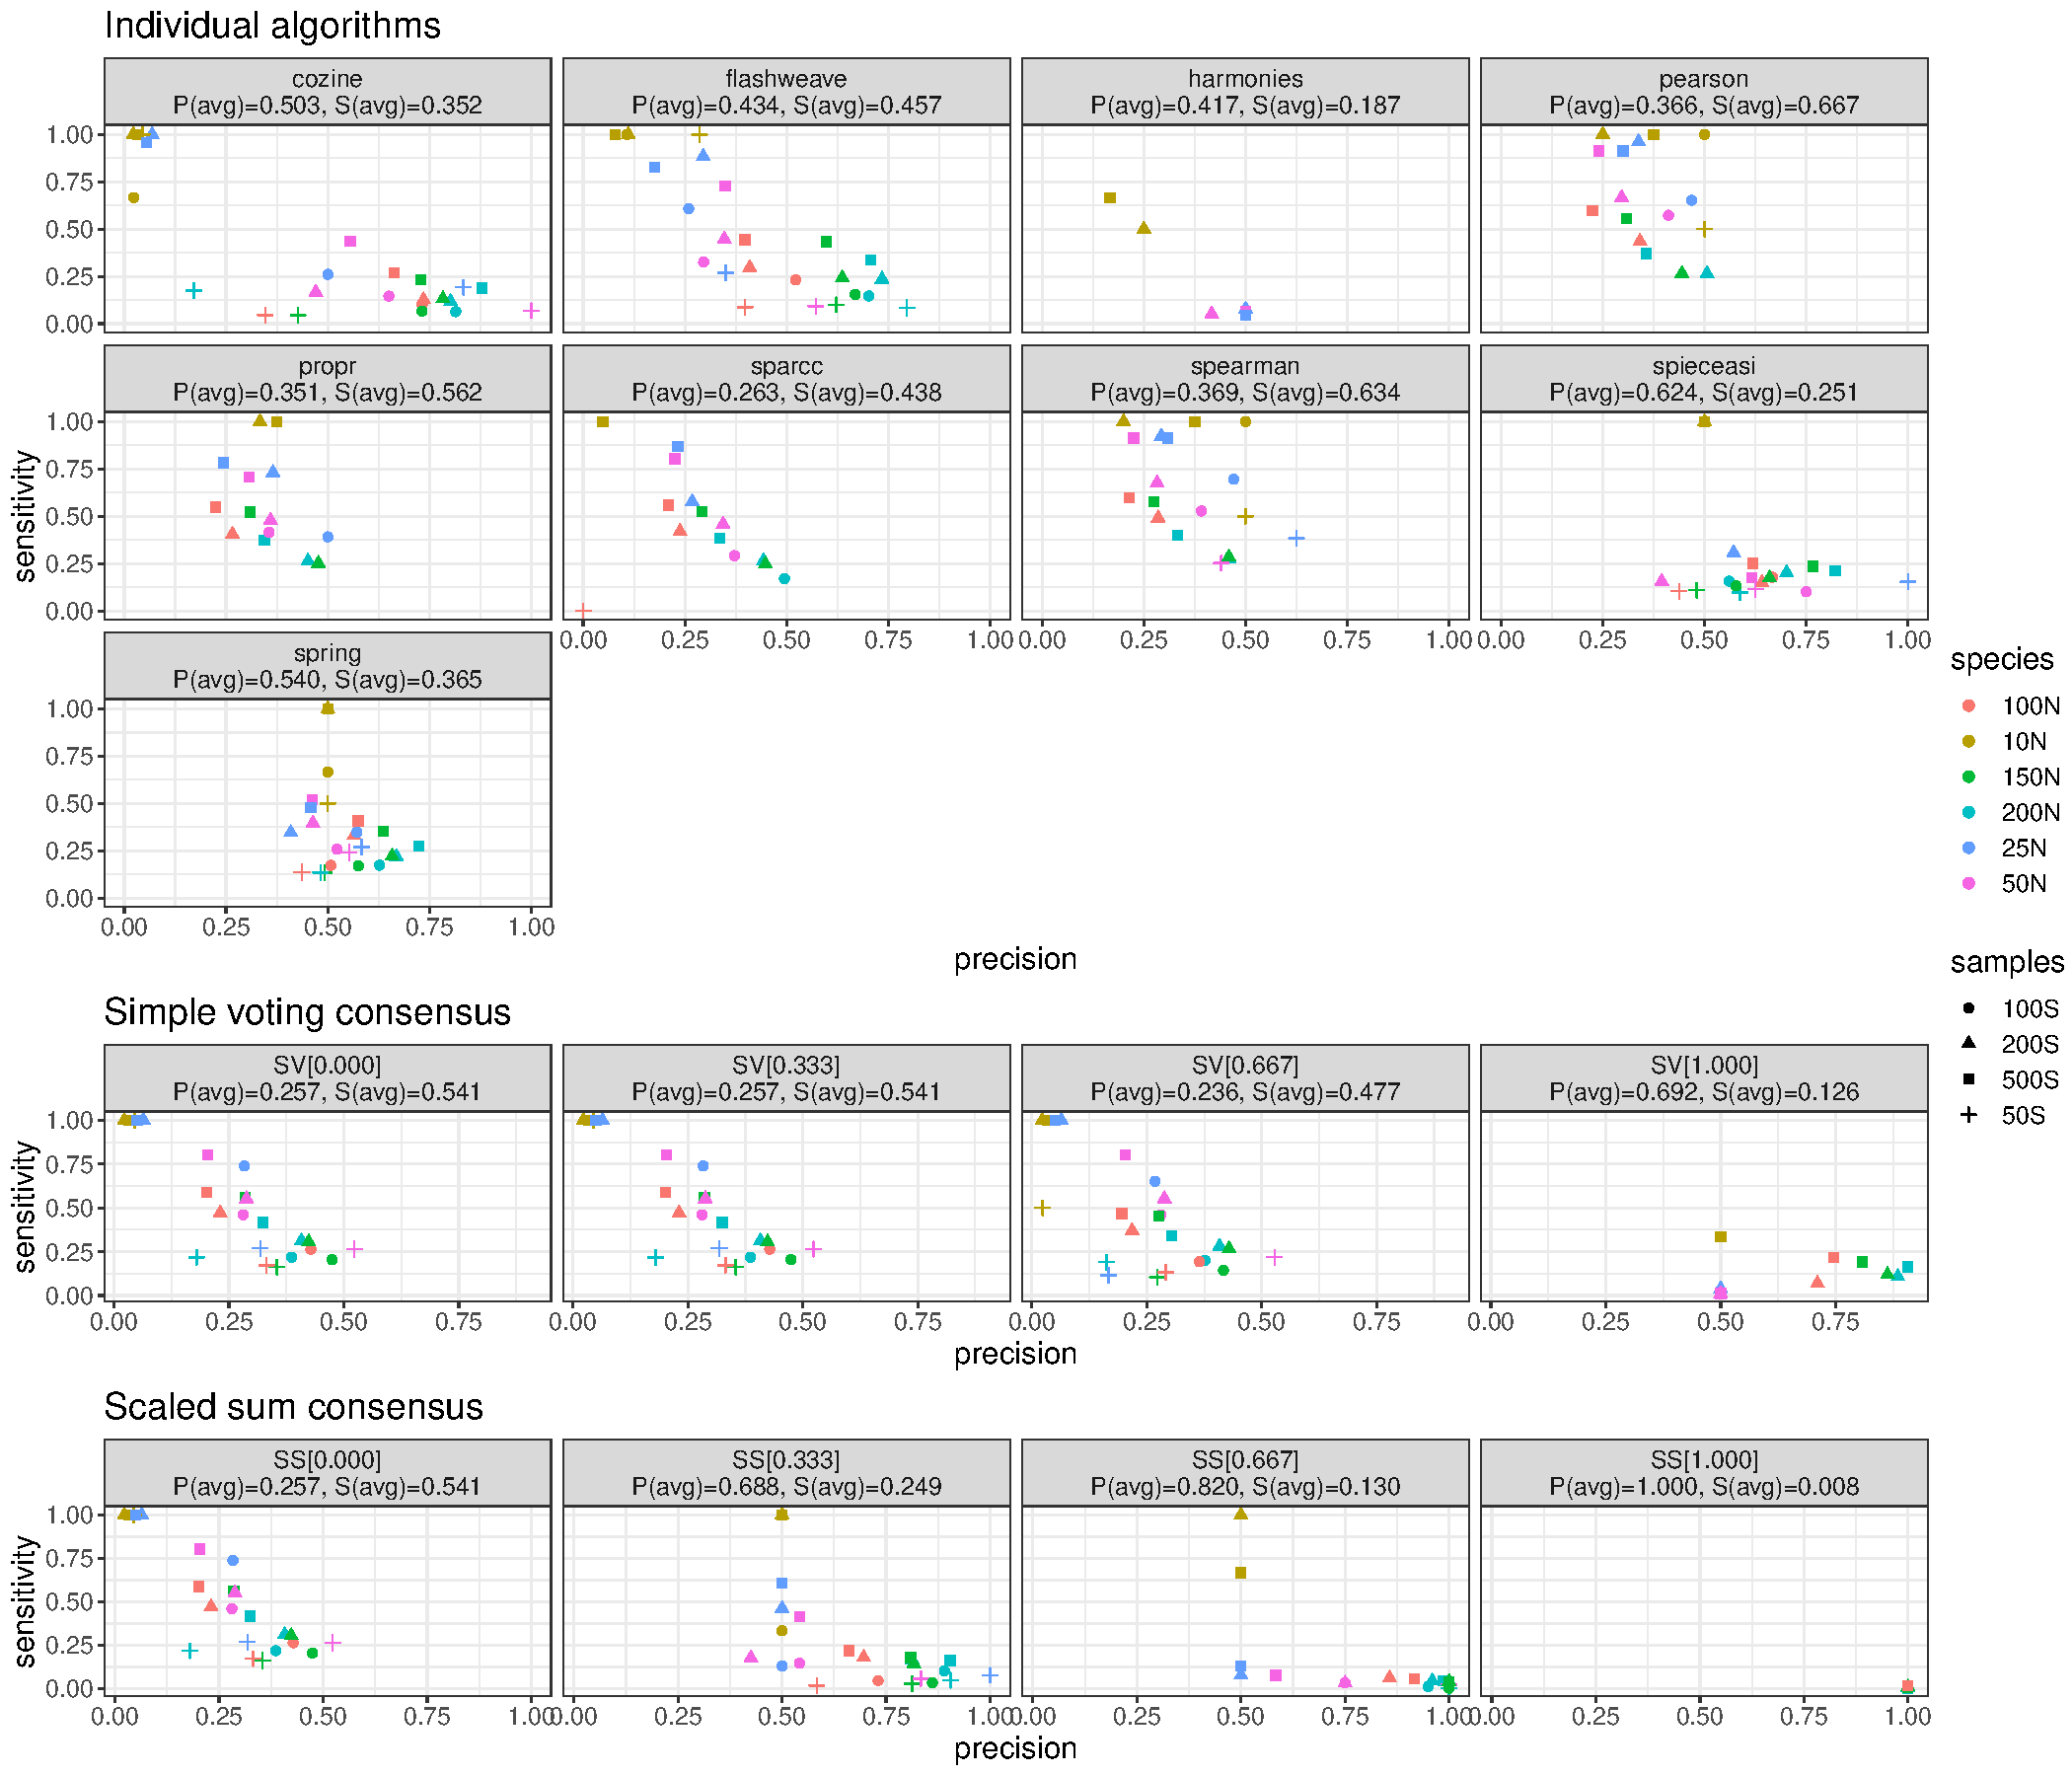
\includegraphics[width=1.0\linewidth]{figure_s6.pdf}
  % \end{figure}
  \begin{figure}[H]
    \centering
      \caption{
        \textbf{The precision and sensitivity of the inferred networks on the ``seqtime'' synthetic interaction data.}
        The different consensus methods used are scaled-sum (SS) and simple voting (SV) methods.
        Pearson and Spearman methods are not used in the calculation of the consensus.
        Among all the independent network inference methods, \acs{spieceasi} has the best average precision (0.624), but the overall best precision was consistently obtained by the scaled-sum method (0.688, 0.820, and 1.000).
        The simple voting method when using the presence of edges in all inferred networks as a requirement ($p = 1.000$), also outperforms \acs{spieceasi} on average precision (0.692).
        These results show that the scaled-sum method is not only much better suited for inferring robust and accurate interactions from count data generated from network topologies (NorTA), but it is also capable of accurately extracting real associations from Lotka-Volterra simulations.
      }
    \label{fig:figure_s6}
  \end{figure}
  % \FloatBarrier
  % \newpage

  % \begin{figure}[H]
  %   \centering
  %   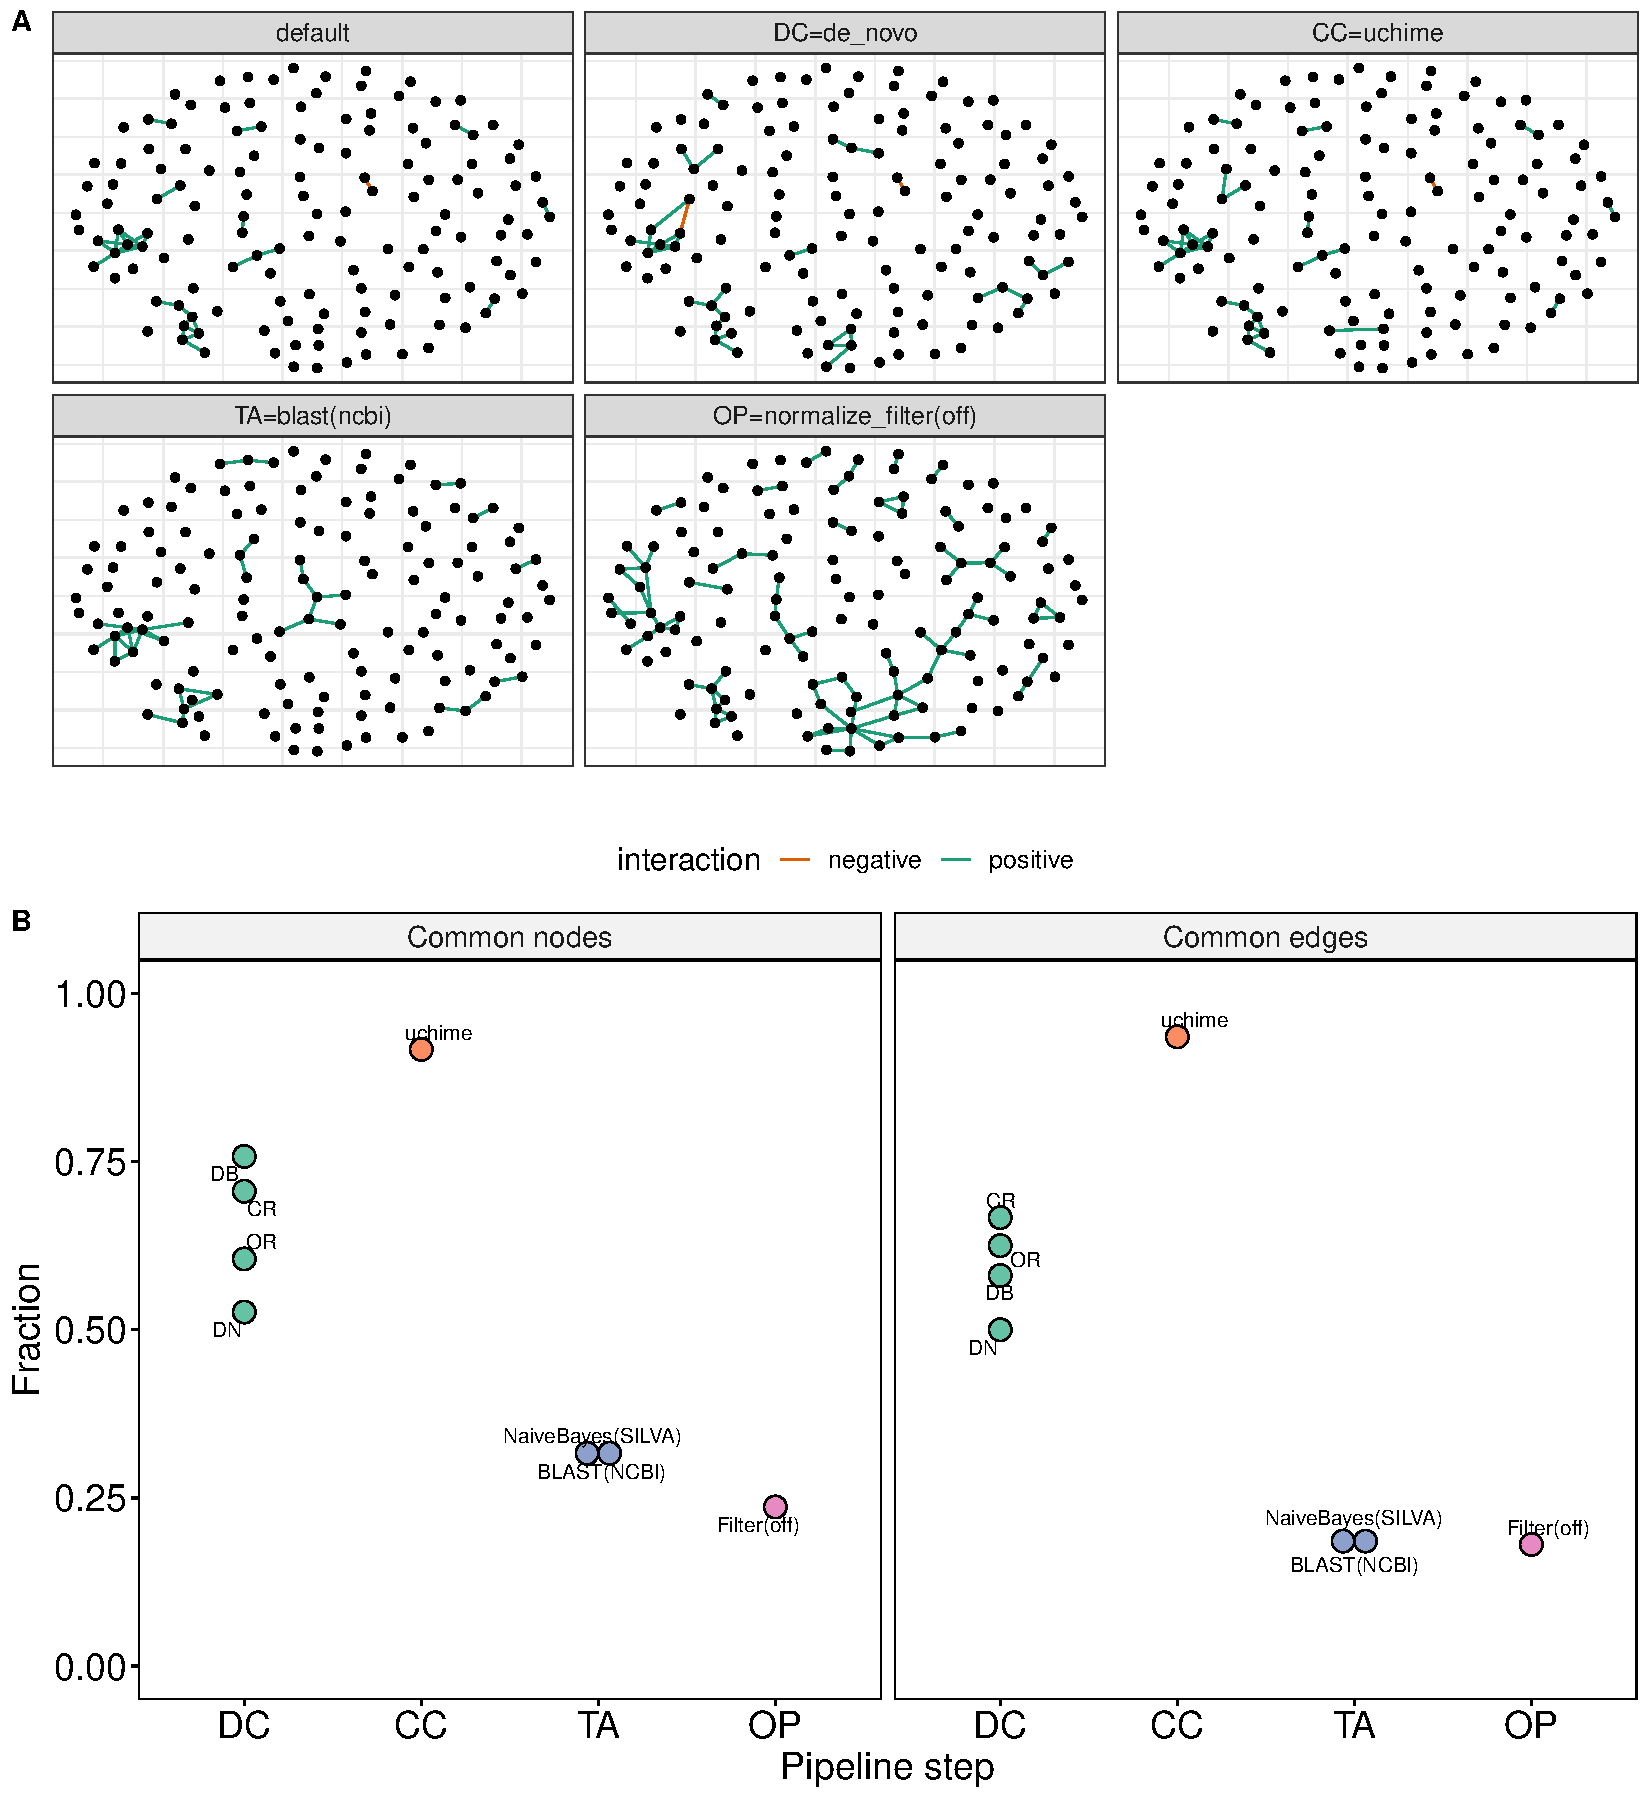
\includegraphics[width=1.0\linewidth]{figure_s7.pdf}
  % \end{figure}
  \begin{figure}[H]
    \centering
    \caption{
      \textbf{Sensitivity analysis of the default settings of the \ac{micone} pipeline}.
      \textbf{(A)} The network constructed using the default pipeline parameters (DC=\ac{dada2}, CC=remove bimera, TA=\ac{gg}, OP=Filter(on), NI=scaled-sum consensus) is compared against networks generated when one of the steps uses a different tool.
      The layout is created by fixing the positions of all the nodes from all networks and then drawing only the relevant edges, making the connections directly comparable.
      The edges colored green are positive associations and those in red are negative associations.
      We observe that changing the TA and OP steps leads to the creation of the most unique edges.
      \textbf{(B)} The dot plot showing the fraction of nodes (left) and edges (right) in common between the default network and the networks generated by changing one step of the default pipeline.
      The low value of the common fraction for TA and OP steps shows that these steps induce the biggest changes in nodes and edges.
      The NI step is not shown in this analysis because the consensus methods use edges from the individual network inference methods and a comparison would be biased.
    }
    \label{fig:figure_s7}
  \end{figure}
  % \FloatBarrier
  % \newpage

